
\documentclass[a4paper,UKenglish,cleveref, autoref, thm-restate]{lipics-v2021}
%This is a template for producing LIPIcs articles. 
%See lipics-v2021-authors-guidelines.pdf for further information.
%for A4 paper format use option "a4paper", for US-letter use option "letterpaper"
%for british hyphenation rules use option "UKenglish", for american hyphenation rules use option "USenglish"
%for section-numbered lemmas etc., use "numberwithinsect"
%for enabling cleveref support, use "cleveref"
%for enabling autoref support, use "autoref"
%for anonymousing the authors (e.g. for double-blind review), add "anonymous"
%for enabling thm-restate support, use "thm-restate"
%for enabling a two-column layout for the author/affilation part (only applicable for > 6 authors), use "authorcolumns"
%for producing a PDF according the PDF/A standard, add "pdfa"

%\pdfoutput=1 %uncomment to ensure pdflatex processing (mandatatory e.g. to submit to arXiv)
\hideLIPIcs  %uncomment to remove references to LIPIcs series (logo, DOI, ...), e.g. when preparing a pre-final version to be uploaded to arXiv or another public repository

%\graphicspath{{./graphics/}}%helpful if your graphic files are in another directory

\bibliographystyle{plainurl}% the mandatory bibstyle

\title{A Compact DAG for Storing and Searching Maximal Common Subsequences} %TODO Please add


\author{Alessio Conte}{Università di Pisa, Italy}{alessio.conte@unipi.it}{https://orcid.org/0000-0003-0770-2235/}{}


\author{Roberto Grossi}{Università di Pisa, Italy}{roberto.grossi@unipi.it}{https://orcid.org/0000-0002-7985-4222/}{}

\author{Giulia Punzi}{National Institute of Informatics, Japan}{punzi@nii.ac.jp}{https://orcid.org/0000-0001-8738-1595/}{}

\author{Takeaki Uno}{National Institute of Informatics, Japan}{uno@nii.ac.jp}{https://orcid.org/0000-0001-7274-279X/}{}

\authorrunning{A. Conte, R. Grossi, G. Punzi, and T. Uno} %TODO mandatory. First: Use abbreviated first/middle names. Second (only in severe cases): Use first author plus 'et al.'

\Copyright{Alessio Conte, Roberto Grossi, Giulia Punzi, and Takeaki Uno} %TODO mandatory, please use full first names. LIPIcs license is "CC-BY";  http://creativecommons.org/licenses/by/3.0/

% \ccsdesc[100]{\textcolor{red}{Replace ccsdesc macro with valid one}} %TODO mandatory: Please choose ACM 2012 classifications from https://dl.acm.org/ccs/ccs_flat.cfm 

% \begin{CCSXML}
% <ccs2012>
%    <concept>
%        <concept_id>10002950.10003624.10003625.10003628</concept_id>
%        <concept_desc>Mathematics of computing~Combinatorial algorithms</concept_desc>
%        <concept_significance>500</concept_significance>
%        </concept>
%    <concept>
%        <concept_id>10002951.10003317.10003371.10003381.10003382</concept_id>
%        <concept_desc>Information systems~Structured text search</concept_desc>
%        <concept_significance>500</concept_significance>
%        </concept>
%    <concept>
%        <concept_id>10002951.10003317.10003371.10003381.10003384</concept_id>
%        <concept_desc>Information systems~Chemical and biochemical retrieval</concept_desc>
%        <concept_significance>500</concept_significance>
%        </concept>
%  </ccs2012>
% \end{CCSXML}

\ccsdesc[500]{Mathematics of computing~Combinatorial algorithms}
\ccsdesc[500]{Information systems~Structured text search}
% \ccsdesc[0]{}


\keywords{Maximal common subsequence, DAG, Compact data structures, Enumeration, Constant amortized time, Random access} %TODO mandatory; please add comma-separated list of keywords

\category{} %optional, e.g. invited paper

\relatedversion{} %optional, e.g. full version hosted on arXiv, HAL, or other respository/website
%\relatedversiondetails[linktext={opt. text shown instead of the URL}, cite=DBLP:books/mk/GrayR93]{Classification (e.g. Full Version, Extended Version, Previous Version}{URL to related version} %linktext and cite are optional

%\supplement{}%optional, e.g. related research data, source code, ... hosted on a repository like zenodo, figshare, GitHub, ...
%\supplementdetails[linktext={opt. text shown instead of the URL}, cite=DBLP:books/mk/GrayR93, subcategory={Description, Subcategory}, swhid={Software Heritage Identifier}]{General Classification (e.g. Software, Dataset, Model, ...)}{URL to related version} %linktext, cite, and subcategory are optional

%\funding{(Optional) general funding statement \dots}%optional, to capture a funding statement, which applies to all authors. Please enter author specific funding statements as fifth argument of the \author macro.

% \acknowledgements{I want to thank \dots}%optional

\nolinenumbers %uncomment to disable line numbering



%Editor-only macros:: begin (do not touch as author)%%%%%%%%%%%%%%%%%%%%%%%%%%%%%%%%%%
\EventEditors{John Q. Open and Joan R. Access}
\EventNoEds{2}
\EventLongTitle{42nd Conference on Very Important Topics (CVIT 2016)}
\EventShortTitle{CVIT 2016}
\EventAcronym{CVIT}
\EventYear{2016}
\EventDate{December 24--27, 2016}
\EventLocation{Little Whinging, United Kingdom}
\EventLogo{}
\SeriesVolume{42}
\ArticleNo{23}
%%%%%%%%%%%%%%%%%%%%%%%%%%%%%%%%%%%%%%%%%%%%%%%%%%%%%%


%%%% OUR PACKAGES %%%%%%

\usepackage{amsmath}
\usepackage{amssymb}
\usepackage{enumerate}
\usepackage{cite}
\usepackage{hyperref}
\usepackage{todonotes}
\usepackage{appendix}
\usepackage{thmtools}
\usepackage{thm-restate}
\usepackage{xspace}

\usepackage{algorithm}
\usepackage{algpseudocode}
\usepackage{caption} 
\usepackage{tikz}
\usetikzlibrary{decorations.pathreplacing, patterns, shapes.geometric}
\tikzstyle{vertex}=[circle, draw, inner sep=0pt, minimum size=6pt]
\tikzstyle{prefixvertex}=[circle, draw, fill = black!25!white, inner sep=0pt, minimum size=6pt]


%%%% OUR COMMANDS %%%%%
\newcommand{\vertex}{\node[vertex]}
\newcommand{\prefixvertex}{\node[prefixvertex]}

\newcommand{\A}{\ensuremath\mathtt{A}}
\newcommand{\C}{\ensuremath\mathtt{C}}
\newcommand{\G}{\ensuremath\mathtt{G}}
\newcommand{\T}{\ensuremath\mathtt{T}}

\newcommand{\oldalg}{\textsc{enumerateMCS}\xspace}
\newcommand{\newalg}{\textsc{CATenumerateMCS}\xspace}
\newcommand{\assessalg}{\textsc{assessMCS}\xspace}
\newcommand{\tswing}[1]{\ensuremath{ \ltimes_T(#1)}\xspace}
\newcommand{\bswing}[1]{\ensuremath {\ltimes_B(#1)}\xspace}
\newcommand{\recID}[4]{\ensuremath{\langle #1, #2, #3, #4 \rangle}\xspace}
\newcommand{\nodelab}[1]{\ensuremath{\mathit{ID}(#1)}\xspace}
\newcommand{\edgelab}[1]{\ensuremath{\ell(#1)}\xspace}
\newcommand{\stpaths}[3]{\ensuremath{\mathcal P_{#1, #2} (#3)}\xspace}
\newcommand{\lbst}[3]{\ensuremath{lb_{#1,#2}  (#3)}\xspace}
\newcommand{\lbrun}{\ensuremath{lb_{\mathit{PD}}}\xspace}
\newcommand{\oracleneigh}[1]{\ensuremath{N^+(#1)}\xspace}
\newcommand{\validext}[1]{\ensuremath{\mathcal{V}(#1)}\xspace}
\newcommand{\activenodes}{\ensuremath{\mathcal{A}}\xspace}
\newcommand{\currsource}{\ensuremath{\mathcal{S}}\xspace}
\newcommand{\MCSDAG}{\textsf{MDAG}\xspace}
\newcommand{\MCSDAGcompr}{\ensuremath{\mathcal{C}}\xspace}
\newcommand{\graphbuild}[1]{\ensuremath{\textsc{buildDAG}(#1)}\xspace}
\newcommand{\MCS}{\ensuremath{\mathit{MCS}\xspace}}
\newcommand{\Ext}{\ensuremath{\mathit{Ext}\xspace}}
\newcommand{\nextc}{\ensuremath{\mathit{next}\xspace}}


\newtheorem{fact}{Fact}



\begin{document}

\maketitle

%TODO mandatory: add short abstract of the document
\begin{abstract}
\emph{Maximal Common Subsequences} (MCSs) between two strings $X$ and $Y$ are subsequences of both $X$ and $Y$ that are maximal under inclusion. MCSs relax and generalize the well known and widely used concept of Longest Common Subsequences (LCSs), which can be seen as MCSs of maximum length. 
%
While the number both LCSs and MCSs can be exponential in the length of the strings, LCSs have been long exploited for string and text analysis, as simple compact representations of all LCSs between two strings, built via dynamic programming or automata, have been known since the '70s.
%
MCSs appear to have a more challenging structure: even listing them efficiently was an open problem open until recently, thus narrowing  the complexity difference between the two problems, but the gap remained significant. 
%
In this paper we close the complexity gap: we show how to build DAG of polynomial size---in polynomial time---which allows for efficient operations on the set of all MCSs such as enumeration in Constant Amortized Time per solution (CAT), counting, and random access to the $i$-th element (i.e., rank and select operations). Other than improving known algorithmic results, this work paves the way for new sequence analysis methods based on MCSs.  
\end{abstract}

\section{Introduction}
\label{sec:introduction}


The \emph{Longest Common Subsequence} (LCS) \cite{stringtostring, survey, hirschberg, fasterlcs} have thoroughly been studied in a plethora of string comparison application domains, like spelling error correction, molecular biology, and plagiarism detection, to name a few. The LCS is a special case of \emph{Maximal Common Subsequence} (MCS) for any two strings $X,Y$: it is a string $S$ that is a subsequence of both $X$ and $Y$, and is inclusion-maximal, namely, no other string $S'$ containing $S$ is also a common subsequence of $X$ and $Y$. The set of all MCSs for $X$ and $Y$ is denoted by $\MCS(X,Y)$. For example, $\MCS(X,Y) = \{\T\A\C\A,\G\}$ for $X = \T\C\A\C\A\G$ and $Y = \G\T\A\C\T\A$, whereas $\T\C\A \not \in \MCS(X,Y)$ as it is contained in $\T\A\C\A$, and the latter is also the only LCS. A crucial observation is the following: if $S$ is a common subsequence, it is always contained in some MCS but this is not necessarily true for LCS (e.g.~$S=\G$ is not contained in $\T\A\C\A$).


In general, LCSs only provide us with information about the longest possible alignment between two strings, while MCSs offer a different range of information, possibly revealing slightly smaller but alternative alignments. For very long strings an MCS may be just slightly shorter than an LCS but provide information on parts of the strings not found by LCSs. In principle, MCS could provide helpful information in all the applications where LCS are used.

While there is a quadratic conditional lower bound for the computation of LCS, based on the Strong Exponential Time Hypothesis~\cite{hardness}, no such bound exists for MCS: actually, an MCS between two strings of length $n$ can be extracted in $O(n\sqrt{\log n /\log\log n})$ time~\cite{SAKAI2019132}.
Moreover it is NP-hard to compute the LCS of an arbitrary number of strings~\cite{maier1978complexity}, whereas a recent polynomial-time algorithm for extracting an MCS from multiple strings exists~\cite{hirota2023fast}.
%
It is worth noting that even though there are a few more different approaches in the literature to find LCS or common subsequences with some kind of constraints (e.g. common subsequence trees \cite{hsu1984computing}, common subsequence automata \cite{crochemore2003directed}), the above observations motivate further investigation to directly deal with MCS. 

In this paper we proceed along that direction, and consider the problem of storing and searching the set $\MCS(X,Y)$. The main hurdle is that $\MCS(X,Y)$ could contain an exponential number of distinct strings~\cite{conte2022enumeration}: consequently, any trie-based or immediate automaton representation
would require \textit{exponential} time and space for its construction. We improve significantly over this direction as we list in our contributions, where $n = \max\{|X|,|Y|\}$ and $\sigma$ is the size of the alphabet $\Sigma$ for $X$ and $Y$:
\begin{itemize}
        \item We introduce a labeled compact direct acyclic graph $\MCSDAG(X,Y)$ (for $MCS$ $DAG$) that represents the strings in $\MCS(X,Y)$ in polynomial space $O(n^3 \sigma)$ and can be built in polynomial time $O(n^3 \sigma \log n)$. 
    \item For any string $P$, we show how $\MCSDAG(X,Y)$ can \textit{search} the strings with prefix $P$ from $\MCS(X,Y)$ and report them in lexicographic order, in $O(|P| \log \sigma + \mathit{occ})$ time, where $\mathit{occ}$ is the number of reported strings.
    \item For any integer $1 \leq i \leq |\MCS(X,Y|$, we show how $\MCSDAG(X,Y)$ with input $i$ can \textit{select} the $i$th string $S$ in lexicographic order from $\MCS(X,Y)$, in $O(|S| \log \sigma)$ time; the inverse operation of \textit{rank} for input $S$ is supported in the same complexity, where $i$ is returned.
    \item We can list all the strings from $\MCS(X,Y)$ lexicographically in constant amortized time (CAT), namely, $O(|\MCS(X,Y)|)$ time.
\end{itemize}

In Section~\ref{section:MCSDAG-construction} we implement $\MCSDAG(X,Y)$ as a direct acyclic graph (DAG) where the only zero indegree node is the source $s$ and the only zero outdegree node is the target $t$. Each edge is labeled with a character from the alphabet, so that any two outgoing edges from the same node have different characters as labels. Moreover, each $st$-path corresponds to a string in $\MCS(X,Y)$, obtained by concatenating the characters on the edge traversed along the $st$-path; vice versa, each string in $\MCS(X,Y)$ is spelled out by an $st$-path. In order to define and build $\MCSDAG(X,Y)$ we use some properties on MCSs previously introduced in~\cite{conte2022enumeration} and described in Section~\ref{section:cat-alg}, plus some new ideas to keep the size of $\MCSDAG$ polynomial. As a result, after $\MCSDAG$ has been built and its unary paths have been compacted, the aforementioned operations can be implemented in a simple way, as shown in Section~\ref{sec:operations}.

Finally, we observe that labels in $\MCSDAG(X,Y)$ may not have constant size each, so of course printing each reported string may require more than constant time. However, our algorithms are able to report a \textit{compressed} form of the output by simply printing the changes, similarly to~\cite{TOMITA200628}. On the other hand, we recall that the complexity of the algorithms should not measure the printing procedures, as formalized by Frank Ruskey~\cite[Section 1.7]{ruskey2003combinatorial} in the ``Don’t Count the Output Principle'', but rather the amount of data change that takes place. As the latter takes constant time per solution, we have CAT complexity. 




\medskip

\noindent\textbf{Related work.} \quad
%
Maximal common subsequences were first introduced in~\cite{first}, in the context of LCS approximation. 
The first algorithm for finding an MCS between two strings was presented in~\cite{Sakai}, and subsequently refined in~\cite{SAKAI2019132}. The latter algorithm finds an MCS between two strings of length $n$ in $O(n\sqrt{\log n /\log\log n})$.
These algorithms can be also used to extend a given sequence to a maximal one in the same time, and to check whether a given subsequence is maximal in $O(n)$ time. 
In~\cite{hirota2023fast} the authors considered the problem of finding an MCS of $m>2$ strings of total length $n$, and were able to solve this in $O(mn\log n)$ time and $O(n)$ space.
As for MCS enumeration,~\cite{conte2022enumeration} showed that this task can be performed in $O(n\log n)$ delay and quadratic space. 



The automaton approach has been used in literature to deal with subsequence-related problems. The Directed Acyclic Subsequence Graph (DASG) introduced in~\cite{baeza1991searching} is an automaton which accepts all subsequences of a given string $S$. 
Given a set of strings, it can also be generalized to accepting subsequences of any string in the set. 
Later, the common subsequence automata (CSA) was introduced~\cite{crochemore1999directed,crochemore2003directed, tronicek2002common}, which instead accepts \emph{common} subsequences of a set of strings. Such automaton is similar to the common subsequence tree of~\cite{hsu1984computing}, and it can also be used to find a longest common subsequence between two strings~\cite{melichar2003longest}. 
%
Binary decision diagrams such as ZDD~\cite{Minato93} and SeqBDD~\cite{LoekitoBP10} could potentially be employed to compactly store $\MCS(X,Y)$ but their worst-case behaviour typically involves exponential construction time and space.

We stress that it is not straightforward to efficiently adapt all of these structures to the MCS problem: indeed, figuring out which of the accepted strings are subsequences of each other is not an immediate task. We therefore opted for a different approach, directly defining and constructing an MCS automaton, based on combinatorial properties specific to MCSs. 


    
\noindent\textbf{Preliminaries. }
%\label{section:prelim}
[\textit{String notation}] 
A string $S$ over an alphabet $\Sigma$ (of size $\sigma=|\Sigma|$) is a concatenation of any number of its characters. The empty string is denoted with $\varepsilon$. For $i \in [0,|S|-1]$, character $S[i]$ occurs at position $i$ of string $S$,
% and position $\nextc_S(i) = j$ is the smallest $j > i$ with $S[j]=S[i]$, if it exists (otherwise,  $\nextc_S(i) = |S|-1$). 
and position $\nextc_S(c, i)$ denote the next occurrence of character $c$ after position $i$ in string $S$, if it exists (otherwise,  $\nextc_S(c,i) = |S|-1$). 
The notation $S_{<i}$ indicates $S[0, i-1]$, and $S_{\leq i}$ indicates $S[0,i]$.
%
    We say that $S$ is a \emph{subsequence} of a string $X$, denoted $S\subset X$, if there exist indices $0\leq i_0 < ... < i_{|S|-1} < |X|$ such that $X[i_k] = S[k]$ for all $k \in [0,|S|-1]$. In this case we also say that $X$ \emph{contains} $S$. Given two strings $X$ and $Y$, a string $S$ is a common subsequence if $S\subset X$ and $S\subset Y$. Furthermore, $S$ is a \emph{Maximal Common Subsequence}, denoted $S \in \MCS(X,Y)$, if it is a common subsequence which is \emph{inclusion-maximal}: there is no string $T \neq S$ such that $S \subset T \subset X,Y$.     
%
\quad [\textit{Graph notation}]
Given a directed graph $G=(V,E)$, we define the in-neighbors of a node $v\in V$  as $N^-(v) = \{u\in V \ | \ (u,v)\in E\}$, and the out-neighbors as $N^+(v) = \{v\in V \ | \ (v,z)\in E\}$; the in-degree is $d^-(v) = |N^-(v)|$ and the out-degree is $d^+(v) = |N^+(v)|$.
%
A subgraph of graph $G= (V,E)$ is a graph $H = (W,F)$ such that $W \subseteq V$ and $F \subseteq E$. 
%
A \emph{path} $P$ in a graph $G= (V,E)$ is a sequence of distinct adjacent nodes: $P = u_1 ... u_k$ where $u_i \in V$ for all $i$, $u_i \neq u_j$ for all $i \neq j$, and $(u_i, u_{i+1})\in E $ for all $i$. $P$ is called an $u_1u_k$-path.  A path where the first and last nodes coincide is called a \emph{cycle}. A directed graph with no cycles is called a directed acyclic graph, or \emph{DAG}. 
%It is folklore that a graph is a DAG if and only if it has a \emph{topological ordering} of its nodes: that is, there is a total ordering of the vertices in $V$ such that if $(u,v)\in E$, then $u < v$ in the ordering. 

\begin{comment}
\paragraph*{Automata notation}
\todo[inline]{not sure how much of this is needed, since we define it as a DAG right away, only commenting that it is an automaton}
\begin{itemize}
    \item A deterministic finite automaton $D$ is a 5-tuple $(Q, \Sigma, \delta, s, F)$ where
    \begin{itemize}
        \item $Q$ is a finite set of states
        \item $\Sigma$ is the alphabet
        \item $\delta: Q \times \Sigma \rightarrow Q$ is the \emph{transition function}
        \item $s\in Q$ is the start state
        \item $F \subseteq Q$ is the set of accepting, or final, states
    \end{itemize}
    We will omit the alphabet $\Sigma$ from the definition, when clear from the context.

    \item A DFA $D$ \emph{accepts} a string $\alpha = c_1,...,c_N$ if there exists a sequence $q_1,...,q_N \in Q$ such that $q_1 = s$, $q_{i+1} = \delta(q_i, c_i)$ for all $1\le i < N$, and $q_N \in F$.

    \item It is easy to see that $D$ can be equivalently represented as an edge-labeled graph, where $Q$ is the set of nodes, and there is an edge between $u,v \in Q$ labeled $c$ if and only if $\delta (u, c) = v$. We will denote such graph as $G(D)$. 
    
    \item $D$ accepts $\alpha$ if and only if there is a path in $G(D)$ from node $s$ to some node in $F$ such that the concatenation of the labels along the edges of the path yield word $\alpha$. We note that if there exists such a path, it is necessarily unique. 



\end{itemize}
\end{comment}



%\subsection{Roadmap}
% We will start, in Section~\ref{section:prelim}, by presenting some string and graph preliminary notions. 

%Section~\ref{section:cat-algo} will present our Constant Amortized Time enumeration algorithm for MCS. First, in Section~\ref{section:automaton-representation}, we will show how to model the problem of MCS enumeration as an instance of $st$-paths enumeration in a DAG, which can be solved in CAT (Section~\ref{sub:cat-stpaths}). 


% Then, we will briefly summarize, in Section~\ref{sec:previous-algo}, algorithm \oldalg from~\cite{conte2022enumeration}. Some notions from \oldalg will be employed to produce our improved CAT algorithm~\newalg, presented in Section~\ref{section:cat-algo}. 
% Finally, Section~\ref{sec:mcs-assessment} will present our assessment algorithm for the number of MCS between two strings. 



\section{Structure of MCSs}
\label{section:cat-alg}

In this section, we show known properties of MCSs which will be at the base of \MCSDAG.
Firstly, we show how to naturally represent all the strings in $\MCS(X,Y)$ for any two given strings $X$ and $Y$, using a finite-state automaton $A$ corresponding to a DAG with a single source $s$ and a single target $t$, where each edge is labeled with a character of the alphabet $\Sigma$; we show that $st$-paths in $A$ have a one-to-one correspondence with the strings in $\MCS(X,Y)$. 
Secondly, we recall and contextualize some useful properties of MCSs proven in~\cite{conte2022enumeration}.

% $\MCSDAG(X,Y)$ with source $s$ and target $t$, whose $st$-paths are in a one-to-one correspondence with the strings in $\MCS(X,Y)$.  After introducing $\MCSDAG(X,Y)$ in Section~\ref{section:automaton-representation}, we detail how to perform its $st$-paths enumeration in constant amortized time (CAT) in Section~\ref{sub:cat-stpaths}. 
% The remainder of the section will describe how to efficiently build an MCS DAG. 
% In the last section, we will discuss the time and space complexity of the presented algorithm. 


\subsection{Modeling MCS as an Exponentially Large DAG}
\label{section:automaton-representation}
% We will start by giving the formal definition of the desired DFA, and some of its properties. From this, we will define the final DAG. 

We here define a deterministic finite-state automaton $A$ that accepts the strings in $\MCS(X,Y)$. It is more convenient to define it directly as an equivalent DAG, using the extended alphabet $\Sigma' = \Sigma \cup \$$, where the dollar sign is a new special character to identify the end of an MCS. 
\begin{definition}
\label{definition:automaton}
The edge-labeled DAG $A = (V\cup \{s,t\},E,\edgelab{\cdot})$
is defined for two input strings $X$ and $Y$ to store their set $\MCS(X,Y)$, as follows:
\begin{itemize}
\item Every node in $V\cup \{s\}$ corresponds to a distinct prefix of a string in $\MCS(X,Y)$, with $s$ called \emph{source node} corresponding to the empty string prefix.
\item For any two nodes $u, u' \in V$, let $P, P'$ be their corresponding two prefixes. Then, $P' = P c$ iff $(u,u') \in E$ with label $\edgelab{u,u'} = c$. 
%That is, an edge from one node to the next means that we can extend the given prefix with the corresponding character label; 
\item For any node $u\in V$, if its corresponding prefix is a whole string $P \in \MCS(X,Y)$, then $(u,t) \in E$ with label $\edgelab{m,t} = \$$. 
%Node $t$ is called the \emph{target node}. %gia detto
\end{itemize}
% Without loss of generality, we use notation $\MCSDAG(X,Y)$ to denote the graph form of the automaton.
\end{definition}

% Finally, we compact the DAG: for each \emph{unary path}, that is, path $u_1...u_k$ such that $N^+(u_i) = \{u_{i+1}\}$ for each $i$, we replace it with the single edge $(u_1,u_k)$, with label $\edgelab{u_1,u_k} = \edgelab{u_1,u_2}\edgelab{u_2,u_3}...\edgelab{u_{k-1},u_k}$.


% Figure environment removed


% \begin{example}
% \label{example:mcsdag}
% Consider strings $X=$\texttt{ACAGTCGT} and $Y=$\texttt{AGTCATGC}.  

% \begin{minipage}{0.6\textwidth}
% The maximal common subsequences of these strings are $\MCS(X,Y) = \{\texttt{AGTCT}, \texttt{AGTCG}, \texttt{ACATG}, \texttt{ACATC}, \texttt{ACAGC}\}$.
% Figure~\ref{fig:MCS-DAG} shows a possible MCS DAG $\MCSDAG(X,Y)$. Note that $d^+(u) \ge 2$ for each node $u$, since unary paths have been compressed. 
% We can see how each string $M \in \MCS(X,Y)$ corresponds to exactly one labeled $st$-path. For example, the topmost $st$-path corresponds to $M = \texttt{ACAGC}$, obtained by concatenating the edge labels along the path. 
% \end{minipage}
% \hfill
% \begin{minipage}{0.3\textwidth}
% \begin{tikzpicture}
%         \vertex[scale = 2] (s) at (0,0) {\tiny $s$};
%         \vertex[scale = 2] (1) at (1,0) {\tiny $1$};
%         \vertex[scale = 2] (2) at (2,1.5) {\tiny $2$};
%         \vertex[scale = 2] (3) at (2,-1.5) {\tiny $4$};
%         \vertex[scale = 2] (4) at (2,0) {\tiny $3$};
%         % \vertex[scale = 2] (5) at (3,0.5) {\tiny $5$};
%         % \vertex[scale = 2] (6) at (3.5,-0.5) {\tiny $6$};
%         % \vertex[scale = 2] (7) at (3.5,-1.5) {\tiny $7$};
%         % \vertex[scale = 2] (8) at (4,2) {\tiny $8$};
%         % \vertex[scale = 2] (9) at (4,1) {\tiny $9$};
%         \vertex[scale = 2] (t) at (4,0) {\tiny $t$};

%         \path[->] 
%         (s) edge node [above] {\texttt{A}} (1)
%         (1) edge[bend left = 10] node [left] {\texttt{CA}} (2)
%         (1) edge[bend right = 10] node [left] {\texttt{GTC}} (3) 
%         (2) edge node [left] {\texttt{T}} (4)
%         (2) edge[bend left = 10] node [above] {\texttt{GC\$}} (t)
%         (3) edge[bend right = 10] node [left] {\texttt{G\$}} (t)
%         (3) edge[bend right = 30] node [below] {\texttt{T\$}} (t)
%         (4) edge[bend left = 10] node [above] {\texttt{C\$}} (t) 
%         (4) edge[bend right = 10] node [below] {\texttt{G\$}} (t) 
%         % (5) edge[bend right = 10] node [above] {\$} (t)
%         % (6) edge[bend right = 10] node [below] {\$} (t)
%         % (7) edge[bend right = 20] node [below] {\$} (t)
%         % (8) edge[bend left = 20] node [above] {\$} (t)
%         % (9) edge[bend left = 10] node [above] {\$} (t)
%         ;
%     \end{tikzpicture}
% \captionof{figure}
% {
% DAG $\MCSDAG(X,Y)$.
% % A possible MCS DAG between strings $X=$\texttt{ACAGTCGT} and $Y=$\texttt{AGTCATGC}. We have $\MCS(X,Y) = \{\texttt{AGTCT}, \texttt{AGTCG}, \texttt{ACATG}, \texttt{ACATC}, \texttt{ACAGC}\}$, and each such string corresponds to exactly one labeled $st$-path. 
% }
% \label{fig:MCS-DAG}
% \end{minipage}


% \end{example}

% \begin{definition}
% An \emph{MCS DFA} for two input strings $X$ and $Y$ is a DFA $A(X,Y) = (Q,\Sigma, \delta, s, F)$  where
% \begin{itemize}
% \item Every state in $Q$ corresponds to a prefix of an MCS of $X$ and $Y$, with $s$ corresponding to the empty string prefix;
% \item Final states $F$ correspond to MCS of $X$ and $Y$;
% \item Let $q, q' \in Q$ be two states, respectively corresponding to prefixes $P, P'$. Then, we have $\delta(q, c) = q'$ if and only if $P' = P c$. That is, we transition from one state to another by extending the given prefix with a character. 
% \end{itemize}
% % Without loss of generality, we use notation $\MCSDAG(X,Y)$ to denote the graph form of the automaton. 
% \end{definition}

% % Figure environment removed

% RG - I think it can be evinced this: As the name suggests, the MCS DAG is acyclic. Indeed, when we move from a state to the next we are extending prefixes by adding new characters. Therefore, when starting from a given node, there is no way of returning to it by following transitions. 


% Given the graph form of an MCS DFA $G(A(X,Y))$, we have a bijection between maximal common subsequences of $X$ and $Y$, and labeled paths from start node $s$ to any node in $F$. 
Given DAG $A$, we have a bijection between the strings in $\MCS(X,Y)$ and the labeled $st$-paths (see the left of Figure~\ref{fig:MCSDAG} for an example).
Indeed, it is immediate that any such path corresponds to a string in $\MCS(X,Y)$ due to the way edges are placed. Vice versa, by definition, we cannot have two out-going edges from the same node that share the same label. Therefore, each MCS has exactly one corresponding $st$-path. 
%
Note that the property of the outgoing labels also implies that $d^+(u) \le  \sigma$ for all $u \in V$, and therefore $|E| \le \sigma |V|$. As the number of nodes in $A$ is $\Omega(|\MCS(X,Y)|)$, its size is exponential in the worst case. 
% since the automaton is deterministic each MCS has exactly one such corresponding path. 

% We are now ready to define the final DAG, over which our algorithm will run:
% \begin{definition}
% Given an MCS DFA $A(X,Y) = (Q,\Sigma, \delta, s, F)$, we define the corresponding \emph{MCS DAG} $\MCSDAG(X,Y) = (V,E,\edgelab{\cdot})$ as the edge-labeled graph obtained as follows:
% \begin{enumerate}
% \item Start with $\MCSDAG(X,Y) = G(A(X,Y))$ the graph form of the MCS DFA, where the edge labels are given by the transition function: $\edgelab{u,v} = c$ if and only if $\delta(u,c) = v$. 
% \item add a new node $t$, and and edges from each node of $F$ to $t$, labeled with the empty string;
% \item for each \emph{unary path}, that is, path $u_1...u_k$ such that $N^+(u_i) = \{u_{i+1}\}$ for each $i$, substitute it with the single edge $(u_1,u_k)$, with label $\edgelab{u_1,u_k} = \edgelab{u_1,u_2}\edgelab{u_2,u_3}...\edgelab{u_{k-1},u_k}$.
% \end{enumerate}
% \end{definition}
% Since $G(A(X,Y))$ is a DAG, it is immediate to see that the resulting MCS DAG is also a acyclic. Furthermore, strings in $\MCS(X,Y)$ still correspond to labeled $st$-paths of $\MCSDAG(X,Y)$.

%RG - maybe we can skip this: Therefore, enumerating the set $\MCS(X,Y)$ is equivalent to enumerating $st$-paths in $\MCSDAG(X,Y)$. The rest of the section is devoted to efficiently performing the latter: we will first present a CAT enumeration algorithm for $st$-paths in a DAG in Section~\ref{sub:cat-stpaths}, and then, after presenting some necessary concepts in Section~\ref{sec:previous-algo}, we will show how we can efficiently build an MCS DAG for two given strings in Section~\ref{section:build-mcs-dag}.



\begin{remark}
$A$ can be seen as an acyclic deterministic finite-state automaton that accepts the set $\MCS(X,Y)$. We have one state for each prefix of a string in $\MCS(X,Y)$. Given two states $q, q'$, respectively corresponding to prefixes $P, P'$ of strings in $\MCS(X,Y)$, % such that $P$ is prefix of $P'$,
the transition function $\delta$ is given by $\delta(q, c) = q'$ if and only if $P' = P c$.
\end{remark}

% \subsection{Path compression phase}
% One more preprocessing step is needed to achieve efficient MCS enumeration. Namely, to achieve CAT complexity we must ensure that all nodes have out-degree greater than 1.  We do this in linear time in the size of the MCS DAG, in the following way. 

% Let us proceed in topological order of the nodes.
% When a node $v$ with $N^+(v) = \{w\}$ (i.e. out-degree 1) is encountered, we perform the following:
% \begin{enumerate}
%     \item For each $u \in N^-(v)$, remove edge $(u,v)$ and add edge $(u, w)$ with label $\edgelab{u,v}\edgelab{v,w}$.
%     \item After all in-neighbors have been processed, remove node $v$ and edge $(v,w)$ from the graph. 
% \end{enumerate}
% Let \MCSDAGcompr be the graph obtained after this procedure. Clearly, the minimum out-degree of this graph is 2.
% % such graph has no nodes of out-degree 1.
% Furthermore, we note that nodes $s$ and $t$ are never removed. It is immediate to see that labeled $st$-paths in \MCSDAG are the same as labeled $st$-paths in \MCSDAGcompr.


\subsection{Known Concepts on MCS Enumeration}
\label{sec:previous-algo}
We now present a summary of some concepts introduced in~\cite{conte2022enumeration}, which will be used for our results. %algorithm \oldalg. 
%
% \paragraph*{String Bipartite Graph}
% A pair of strings $X,Y$ is seen as a graph, called \emph{string bipartite graph}. Such graph has a node $x_i$ (resp. $y_j$) for every position $i$ (resp. $j$) of string $X$ (resp. $Y$). Edge $(x_i,y_j)$ belongs to the graph if and only if $X[i] = Y[j]$. For ease of notation, we will denote edge $(x_i,y_j)$ simply as $(i,j)$.
% %
% On this bipartite graph, a \emph{mapping} is defined as a matching whose edges never cross. That is, if $(i,j)$ and $(h,k)$ belong to the matching, then we have $i < h$ if and only if $j < k$. Every mapping corresponds to a common subsequence of $X$ and $Y$.
% We stress that, as shown in~\cite{conte2022enumeration}, inclusion-maximal mappings \emph{do not} correspond to MCSs. 
% An important concept to prove maximality of a subsequence is the following definition. 
% % \begin{definition}
% % \label{def:left-right-mapping}
% A mapping $\mathcal M$ of $G(X,Y)$ is called \emph{rightmost} if for each edge $(i,j)\in \mathcal M$,
% % corresponding to character $c \in \Sigma$, 
% the next edge $(i',j')$ of the mapping satisfies $\nextc_X(i)\geq i'$ and $\nextc_Y(j)\geq j'$. 
% % That is, there are no occurrences of $c$ in $X[i+1, \dots, i'-1]$ and $Y[j+1, \dots, j'-1]$, the portions between edges $(i,j)$ and $(i',j')$. 
% We can symmetrically define a \emph{leftmost} mapping.
% % \end{definition}
% In other words, if we look at the subsequence spelled by a leftmost (resp. rightmost) mapping, the edges of the mapping identify the occurrence of the sequence that is leftmost (resp. rightmost) in both strings $X$ and $Y$. See the left of Figure~\ref{fig:swings} for an example.
% \begin{example}
% \label{example:mappings}
% Consider again $X=$\texttt{ACAGTCGT} and $Y=$\texttt{AGTCATGC}, as in Example~\ref{example:mcsdag}. 
%   ***EXAMPLE***
% \end{example}
%
% The final central concept is the one of \emph{unshiftable edges}:
% \begin{definition}
% An edge $(i,j)$ of the bipartite graph $G(X,Y)$ is  \emph{unshiftable} if it belongs to at least one maximal rightmost mapping of $G(X,Y)$. The set of unshiftable edges is denoted $\mathcal U$. 
% \end{definition}
% The idea behind unshiftable edges is that they belong to at least one (maximal) mapping where nothing can be inserted between the corresponding character and the next.
% %
% The authors of~\cite{conte2022enumeration} show that unshiftable edges can be  $O( n^2 )$, where $n = \max \{|X|,|Y|\}$, and they present a $O(\sigma n^2 \log n)$-time algorithm to find all unshiftable edges given $X$ and $Y$. 
%\paragraph*{Algorithm \oldalg}
% Algorithm \oldalg is proposed in~\cite{conte2022enumeration} to enumerate the strings in $\MCS(X,Y)$. Its general scheme is a binary partition procedure, where increasingly long prefixes of MCSs are built. More specifically, 
Let string $P$ be called a \emph{valid prefix} if there exists a string $Q$ such that their concatenation is $PQ\in \MCS(X,Y)$. Given a valid prefix $P$, the set of characters $c$ such that $P \, c$ is still a valid prefix are called \emph{valid extensions}. 
% A key ingredient is set of \emph{candidate extensions}, intuitively a subset of $\Sigma$ that makes sense to consider to extend $P$; this is computed in~\cite{conte2022enumeration} from $\Ext_{l,m}\subseteq \{0,...,n\} \times \{0,...,n\}$, which has size $O(\sigma)$, and can be found in $O(\sigma \log n)$ time (see~\cite[Section 2.3]{conte2022enumeration}). More importantly, it depends only on the values of $l$ and $m$ and the given $X, Y$.
% only depends on the values of $l$ and $m$ and the given $X, Y$; more details are beyond the scope of this paper, but they can be found in~\cite[Section 2.3]{conte2022enumeration}, along with a method showing how to get it in $O(\sigma \log n)$ time. 

Finding valid extensions of $P$ is not straightforward.
Let $P$ be a valid prefix, and let $X_{\le l}$ and $Y_{\le m}$ be respectively the shortest prefixes of $X$ and $Y$ that contain $P$ as a subsequence. Consider a pair of positions $i > l$ and $j > m$, respectively in $X$ and $Y$, corresponding to the same character, say,~$c \in \Sigma$. In order to assess whether $c$ is a valid extension, checking if $P \, c$ is a maximal common subsequence of $X_{\le i}$ and $Y_{\le j}$ is necessary, but not sufficient: 


\begin{example}
\label{exa:pitfall}
Consider $X = \texttt{TCACAG}$ and $Y = \texttt{TACGAT}$, with $\MCS(X,Y ) = \{\texttt{TACA}, \texttt{TACG}\}$.

\noindent\begin{minipage}{.3\textwidth}
    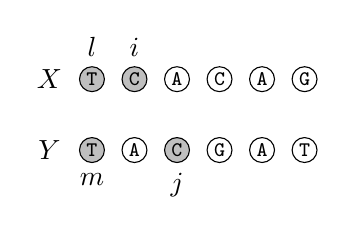
\begin{tikzpicture}[square/.style={regular polygon,regular polygon sides=4},x=.6cm, y=1cm, scale = 0.9]
\node at (-1,1) {$X$};
    \prefixvertex[scale = 1.5] (xbeg) at (0,1) [label = above:  $l$] {\tiny \texttt{T}};
    \prefixvertex[scale = 1.5] (x1) at (1,1) [label = above:  $i$] {\tiny \texttt{C}};
    \vertex[scale = 1.5] (x2) at (2,1) {\tiny \texttt{A}};
    \vertex[scale = 1.5] (x3) at (3,1) {\tiny \texttt{C}};
    \vertex[scale = 1.5] (x4) at (4,1) {\tiny \texttt{A}};
    \vertex[scale = 1.5] (x5) at (5,1)   {\tiny \texttt{G}};
    
\node at (-1,0) {$Y$};  
    \prefixvertex[scale = 1.5] (ybeg) at (0,0) [label = below:  $m$] {\tiny \texttt{T}};
    \vertex[scale = 1.5] (y1) at (1,0) {\tiny \texttt{A}};
    \prefixvertex[scale = 1.5] (y2) at (2,0) [label = below:  $j$] {\tiny \texttt{C}};
    \vertex[scale = 1.5] (y3) at (3,0)  {\tiny \texttt{G}};
    \vertex[scale = 1.5] (y4) at (4,0) {\tiny \texttt{A}};
    \vertex[scale = 1.5] (y5) at (5,0)  {\tiny \texttt{T}};
   
    \path
        % (xbeg) edge[color = black, line width = 1pt] (ybeg)
        % (x1) edge[color = black, line width = 1pt] (y2)
        % (x3) edge[color = black, line width = 1pt] (y3)
        % (x4) edge[dashed, color = black, line width = 1pt] (y4)
        % (x6) edge[dashed, color = black, line width = 1pt] (y5)
        % (x5) edge[dashed, color = black, line width = 1pt] (y7)
        % (x7) edge[dashed, color = black, line width = 1pt] (y6)
        % 
        ;
\end{tikzpicture}
\end{minipage}
\begin{minipage}{.66\textwidth}
     Consider the valid prefix $\T$, for which $l=0$ and $m=0$. Let $i=1$ and $j = 2$: these correspond to character $\C$, and clearly $\T\C \in \MCS(X_{\le i}, Y_{\le j}) = \MCS(\texttt{TC}, \texttt{TAC})$. Still, $\C$ is not a valid extension of valid prefix $\T$, as $\T\C$ is not a prefix of any MCS. 
\end{minipage}
\end{example}

% see Figure~\ref{fig:swings} as a counterexample.
% One may think that valid extensions could be identified by considering the next occurrences $i = \nextc_X(c,l)$ and $j = \nextc_Y(c,m)$ of a character $c \in \Sigma $ after positions $l$ and $m$, such that no other $d \in \Sigma$ occurs before both $i$ and $j$. Unfortunately, this does not suffice: see the left of Figure~\ref{fig:swings} as a couterexample. 
To circumvent this problem, the set $\Ext_{l,m}$ of \emph{candidate extensions} is defined in~\cite{conte2022enumeration}: this is a set of pairs of positions $(i,j)$, with $i \ge l$ and $j \ge m$, whose definition relies solely on the pair $(l,m)$. The membership of $(i,j)$ to $\Ext_{l,m}$ completes the characterization of valid extensions (see Theorem 3 in~\cite{conte2022enumeration}): 
% which can be computed in $O(\sigma \log n)$; we omit the detailed procedure which is not relevant, but it can be found in~\cite[Section 2.3]{conte2022enumeration}. Intuitively, $\Ext_{l,m}$ will contain one edge for each possible extending character in $\Sigma$, as long as it respects some combinatorial properties.
% Valid extensions are characterized as follows (see Theorem 3 in~\cite{conte2022enumeration}):
\begin{itemize}
    \item Let $P$ be a valid prefix, and let $X_{\le l}$ and $Y_{\le m}$ be respectively the shortest prefixes of $X$ and $Y$ that contain $P$ as a subsequence.
    % of some $M \in \MCS(X,Y)$, 
    % with leftmost mapping $L_P$ ending with edge $(l,m)$. 
    \item Then $P\, c$ is a valid prefix if and only if the following two conditions hold:
    \begin{enumerate}
        \item \label{condition:swings} There exists $i$ and $j$ such that $c = X[i] = Y[j]$ and  $P \in \MCS(X_{<i}, Y_{<j})$;
        \item \label{condition:ext} This pair of positions satisfies $(i,j) \in \Ext_{l,m}$.
    \end{enumerate} 
\end{itemize}
More details on the construction of set $\Ext_{l,m}$ are beyond the scope of this paper, but they can be found in~\cite[Section 2.3]{conte2022enumeration}, along with a  $O(\sigma \log n)$ time method for its computation. In Example~\ref{exa:pitfall}, it is $(i,j) \not \in \Ext_{l,m}$.

% At every step, a valid prefix $P$ is given, and all distinct characters $c$ such that $P \, c$ is still a valid prefix are identified by the algorithm. \oldalg recurs over all these new prefixes, which will clearly lead to distinct MCSs.
% To be able to identify characters that extend $P$ in a valid way, called \emph{valid extensions}, a suitable set of edges is called \emph{candidate extensions}, denoted $\Ext_P$. The formal definition of this set is beyond the scope of this paper, but it can be found in~\cite[Section 2.3]{conte2022enumeration}, along with a method showing how to efficiently extract such set, given only the last edge of the leftmost mapping of $P$, in $O(\sigma \log n)$ time. 

% % , which we will describe in detail in Section~\ref{section:unshift-candidate}. 
% Using this set, valid extensions are characterized as follows (see Theorem 3 in~\cite{conte2022enumeration}):
% \begin{itemize}
%     \item Let $P$ be a valid prefix 
%     % of some $M \in \MCS(X,Y)$, 
%     with leftmost mapping $L_P$ ending with edge $(l,m)$. 
%     \item Then $P\, c$ is a valid prefix if and only if the following two conditions hold:
%     \begin{enumerate}
%         \item There exists $(i,j) \in \Ext_P$ corresponding to character $c$, and
%         \item $P \in \MCS(X_{<i}, Y_{<j})$.
%     \end{enumerate} 
% \end{itemize}
% %
 
% \subsection{Unshiftable edges and Candidates' set}
% \label{section:unshift-candidate}
% Unshiftable edges are used to define the candidate extensions set $\Ext_P$ as follows. Given an edge $(l,m)$, its \emph{cross} $\chi_{(l,m)} = \langle e,f \rangle$ is given by (at most) two unshiftable edges $e = (e_1,e_2), f=(f_1,f_2)$ that come ``right after'' $(l,m)$. 
% % These are shown in purple in Figure~\ref{fig:ext}. 
% Formally, we can define $e_1 = \min \{h_1>l \ | \ \exists h_2 > m \text{ : } (h_1,h_2) \in \mathcal U \}$, and $e_2 = \min\{h_2 >m : (e_1, h_2) \in \mathcal U\}$ for the first edge, and $f_2 = \min \{h_2>m\ | \ \exists h_1 > l \text{ : } (h_1,h_2) \in \mathcal U \}$ and $f_1 = \min\{h_1 >l : (h_1, f_2) \in \mathcal U\}$ for the second edge (see the purple edges in the left of Figure~\ref{fig:ext}).
% % \begin{align*}
% %     e_1 &= \min \{h_1>l \ | \ \exists h_2 > m \text{ : } (h_1,h_2) \in \mathcal U \} &\ \text{and } e_2 = \min\{h_2 >m : (e_1, h_2) \in \mathcal U\} \\
% %     f_2 &= \min \{h_2>m\ | \ \exists h_1 > l \text{ : } (h_1,h_2) \in \mathcal U \} &\text{and } f_1 = \min\{h_1 >l : (h_1, f_2) \in \mathcal U\}.
% % \end{align*}
% % \[e_1 = \min \{h_1>l \ | \ \exists h_2 > m \text{ : } (h_1,h_2) \in \mathcal U \} \text{ and } e_2 = \min\{h_2 >m : (e_1, h_2) \in \mathcal U\},\] 
% % \[f_2 = \min \{h_2>m\ | \ \exists h_1 > l \text{ : } (h_1,h_2) \in \mathcal U \} \text{ and } f_1 = \min\{h_1 >l : (h_1, f_2) \in \mathcal U\}.\]
% %
% %
% From this, the \emph{mikado edges} are defined as the unshiftable edges with both endpoints in subgraph $G(X[e_1,...,f_1], Y[f_2,...,e_2])$, 
% % \[Mk_{(l,m)} = \{(i,j) \in \mathcal U \ | \ e_1 \leq i \leq f_1 \text{ and } f_2 \leq j \leq e_2\},\]
% and finally we can define (see the left of Figure~\ref{fig:ext})
% % the subset of \emph{candidate extensions} for $(l,m)$ as 
% \[\Ext_{(l,m)} = \{(i,j) \in Mk_{(l,m)} \ | \ \not \exists (h,k) \in Mk_{(l,m)} \setminus (i,j) \text{ such that } h \leq i \text{ and } k\leq j\}.\]

% We can use notation $\Ext_{(l,m)}$ instead of $\Ext_P$, since the set only depends on the last edge of the corresponding leftmost mapping. 
% %
% Note that, by definition, all edges in $\Ext_{(l,m)}$ have distinct endpoints. In~\cite{conte2022enumeration}, the authors show how to compute this set in $O(\sigma \log n)$ time. 




% % Figure environment removed


% Figure environment removed




% \subsection{Swings for Maximality Check}
The notion of \emph{swings} is a key concept to quickly verify the first condition above. Swings characterize the amount by which we can ``move'' a given character occurrence while retaining maximality (see Figure~\ref{fig:swings}, right). 
Let $X_{\le l}$ and $Y_{\le m}$ be respectively the shortest prefixes of $X$ and $Y$ that contain $P$ as a subsequence. 
% a leftmost mapping for some string $P$, ending with edge $(l,m)$. 
The \emph{swing} of $P$, denoted $\ltimes(P)$, is a pair of integers  $\ltimes_T(P)$ and $\ltimes_B(P)$, called respectively \emph{top} and \emph{bottom} swings, given by
\begin{itemize}
    \item $\ltimes_T(P) = \min \{ i> l \ | \ P \not \in \MCS(X_{\le i},Y_{\le m})\}$ %= \max \{ i> l \ | \ P \in \MCS(X_{< i},Y_{\le m})\}
    \item $\ltimes_B(P) = \min \{j>m \ | \ P \not \in \MCS(X_{\le l},Y_{\le j})\}$ %= \max \{ j> m \ | \ P \in \MCS(X_{\le l},Y_{< j})\}
\end{itemize}
It follows from the definition that $P \in \MCS(X_{< i}, Y_{< j}) \iff i \le \ltimes_T (P) \text{ and } j \le  \ltimes_B(P)$. Given the swings, condition~\ref{condition:swings} can thus be checked in constant time~\cite{conte2022enumeration}. 

% \paragraph*{Incremental Computation of Swings}
% Therefore, we can check in constant time if the swings are computed as the algorithm proceeds.
Updating the swings when a character is added can be done in $O(\sigma)$ time, provided that we can find in constant time the next occurrence of a character $c$ after a given position in the strings; more importantly, this update does \textit{not} need knowledge of the whole prefix, but just the positions its final character ($l_N,m_N$) and their current swings. 

% It is now crucial to observe that $\Ext_{l,m}$ and the swings are all that is necessary to compute the valid extensions of $P$, and they do \textit{not} depend on $P$. Specifically:

% \begin{remark}
%     The valid extensions of a prefix $P$ can be computed from just knowledge of $l_N,m_N$ and their swings.
% \end{remark}


% % \subsection{Algorithm \oldalg}
% Algorithm \oldalg exploits the two conditions above and the notion of swings: at each step, the leftmost mapping $L$ of a valid prefix $P$ and its swings $\ltimes (L)$ are given. The algorithm computes set $\Ext_P$, and for every character $c$ corresponding to an edge $(i,j)$ in $\Ext_P$: it checks if $i \le \ltimes_T(L)$ and $j \le \ltimes_B(L)$; if so, it computes the leftmost mapping and the swings for string $P\, c$, and recurs. If no characters passed this check, the algorithm outputs $P$ as an MCS.

% All MCS can be output if we start from the empty string $\varepsilon$ as prefix (empty leftmost mapping and swings $\ltimes(\varepsilon) = (|X|,|Y|)$). Overall, the algorithm requires a preprocessing of $O(n^2\log n)$ time, and it has a delay of $O(\sigma n \log n)$. The space employed is quadratic. 
% % every step requires $O(\sigma \log n)$ time, and at most $n$ steps are required to generate an $MCS$.





\section{Polynomial-Size \MCSDAG}
\label{section:MCSDAG-construction}
% The key part our algorithm is how to construct an MCS DAG, given two input strings $X,Y$. In the rest of the paper, we will show how this can be done in $O(n^3 \sigma \log n )$ time and $O(n^3)$ space, concluding the proof of Theorem~\ref{thm:main-CAT}. 
The construction of DAG $A$ satisfying the conditions of Definition~\ref{definition:automaton} would require exponential time and space: the number of nodes of $A$ is between  $\Omega(|\MCS(X,Y)|)$ and $O(n|\MCS(X,Y)|)$, so it can be exponential in $n$. In this section, we show how to obtain $\MCSDAG$, where we still have a bijection between $st$-paths and MCS, but which can instead always be constructed in $O(n^3 \sigma \log n )$ time and $O(n^3\sigma)$ space, as per Theorem~\ref{thm:main-CAT}. Intuitively, the relevant information discussed for $A$
are the quadruples $(l,m, t, b)$, where $X_{\le l}$ and $Y_{\le m}$ are some prefixes and pair $t, b$ is some swing: these quadruples are the candidates for being nodes in $\MCSDAG$.


% After giving an overview of the needed concepts in Section~\ref{sec:previous-algo}, we will present our algorithm for constructing our $\MCSDAG$ in Section~\ref{section:build-mcs-dag}. The complexity bounds for the construction will finally be presented in Section~\ref{section:mcsdag-size}. 
The formal definition of \MCSDAG is based on an equivalence relation over the nodes of $A$, given in Section~\ref{section:mcsdag-eqrel}. 
Afterwards, in Section~\ref{section:mcsdag-construction}, we describe an algorithm for \textit{directly} constructing $\MCSDAG$. We present the complexity bounds for the construction in Section~\ref{section:mcsdag-size}. 

\subsection{Equivalence Relation for Defining \MCSDAG}
\label{section:mcsdag-eqrel}
Let $A$ be a DAG as defined in Definition~\ref{definition:automaton}.
Our construction algorithm for $\MCSDAG$ is based on the concepts from Section~\ref{sec:previous-algo}. 
The idea is to use the characterization of valid extensions to identify the out-neighbors of a given node of DAG $A$. 
% Indeed, given a prefix $P$, the corresponding recursive call of \oldalg allows us to identify, in $O(\sigma \log n)$ time, all the characters that extend $P$ in a valid way. In our MCS DAG, this means identifying all of the out-neighbors of the corresponding node. 
%
%The incremental construction could proceed by extending all the prefixes, but it would require
%
% proceeds as follows. Start with node $s$. At the generic step, pick a node $u$ with out-neighbors to discover, and let $P$ be the corresponding prefix. Compute the valid extensions using swings and the set $Ext$. For each valid extension $c$, add a new neighboring node corresponding to prefix $Pc$, connected to $u$ through an edge labeled with $c$. The problem with this construction is that the graph size is necessarily $|\MCS(X,Y)|$, which can be exponential in the length of the input strings. Therefore, the graph building phase could require 
%
%exponential time and space, in the worst case.  We follow a different path and 
We identify an equivalence relation over the prefixes of $\MCS(X,Y)$, and thus on the nodes of $A$, that allow us to always build $\MCSDAG$ in polynomial time and space.  
%
We begin with the following lemma:
\begin{lemma}
\label{lemma:equal-extensions}
    Given any valid prefix $P$, let $X_{\le l}$ and $Y_{\le m}$ be the shortest prefixes containing $P$, and
    $\ltimes(P) = \langle t, b \rangle$ be its swing. Consider another valid prefix $P'\neq P$ with the \emph{same} shortest prefixes $X_{\le l}, Y_{\le m}$ and swing $\ltimes(P') = \ltimes(P)$ as $P$. Then, the set of valid extensions is the same for both $P$ and $P'$, and for each valid extension $c \in \Sigma$, the swings of $P\, c$ are the same as the ones of $P'\, c$. 
\end{lemma}
\begin{proof}
The definition of $\Ext_{l,m}$ only depends on the value of $l$ and $m$, therefore such set is the same for both $P$ and $P'$. Since the swings form $P$ and $P'$ are equal, the set of valid extensions is necessarily the same. 
%
Let now $c \in \Sigma$ be a valid extension for $P$ and $P'$. Let $X_{\le l_c}$ and $Y_{\le m_c}$ respectively be the shortest prefixes of $X$ and $Y$ containing $P\, c$. These are also the shortest prefixes containing $P' \, c$: the shortest prefixes containing $P$ and $P'$ were the same, and $l_c$ is simply the first occurrence of $c$ after $l$, analogously for $m_c$ and $m$. 
%Recall now the incremental computation of swings: 
The swings of $P \, c$ are given by the minimum of the swings of $P$, and the personal swing $\ltimes{(l_N, m_N)}$ obtained by adding the new character $c$. The latter personal swing is the same for both $P \, c$ and $P'\, c$, since we are considering the same positions $l_c,m_c$. Since the previous swings where also equal, this means that the swings of $P \,c $ and $P' \, c$ are indeed the same. 
\end{proof}

Lemma~\ref{lemma:equal-extensions} has an implication for prefixes $P$ and $P'$ that share the \textit{same} swing: if $M_1,...,M_N$ are strings extending as $PM_i \in \MCS(X,Y)$, and $M'_1,...,M'_M$ extending as $P'M'_i \in \MCS(X,Y)$, then they are equal: $\{M_i \ | \ i = 1,...,N\}=\{M'_i \ | \ i = 1,...,M \}$.


Given a node $u$ of $A$, let $P$ be the corresponding prefix.  We assign $u$ the quadruple of parameters $\nodelab{u} = \langle l,m,\tswing{P}, \bswing{P}\rangle$, where $l$ and $m$ are such that $X_{\le l}$ and $Y_{\le m}$ are the shortest prefixes containing $P$. 
By Lemma~\ref{lemma:equal-extensions}, this tuple completely identifies the valid extensions of $P$, which means that it completely identifies the neighbors of node $u$. 
\begin{corollary}
\label{corollary:same-neighbors}
    Let $u \neq u'$ with $\nodelab{u} = \nodelab{u'}$. Then, for each $v \in N^+(u)$ there exists exactly one $v' \in N^+(u')$ such that $\nodelab{v} = \nodelab{v'}$ and $\edgelab{u,v} = \edgelab{u',v'}$.
\end{corollary} 

Therefore, we can define the following \emph{equivalence relation} on the nodes of $A$: $u \sim u'$
if and only if $\nodelab{u} = \nodelab{u'}$. We can then identify a class of equivalent nodes in the DAG, choosing one representative for it. Because of Corollary~\ref{corollary:same-neighbors}, this does not change the set of labeled $st$-paths of the DAG: the nodes that are identified as one have the same labelled out-edges, leading to the same out-neighbors. Our data structure \MCSDAG is then defined as the DAG resulting from this identification:
\begin{definition}
\label{definition-MCSDAG}
Data structure $\MCSDAG$ is a node- and edge-labelled DAG  built as follows:
\begin{enumerate}
\item Start from DAG $A$ (Definition~\ref{definition:automaton}). For each node $u$, consider its (unique) corresponding prefix $P$, and let $X_{\le l}$ and $Y_{\le m}$ be the shortest prefixes of $X$ and $Y$ containing $P$, and $\ltimes(P) = (t,b)$. Assign to node $u$ the node-label $\nodelab{u}=\recID{l}{m}{t}{b}$. \label{item:MCSDAG-start}
\item Merge every pair of nodes $u \neq u'$ with the same label $\nodelab{u} = \nodelab{u'}$ into one node.  \label{item:MCSDAG-identify}
% \item For each \emph{unary path}, that is, path $u_1...u_k$ such that $N^+(u_i) = \{u_{i+1}\}$ for each $i$, substitute it with the single edge $(u_1,u_k)$, with label $\edgelab{u_1,u_k} = \edgelab{u_1,u_2}\edgelab{u_2,u_3}...\edgelab{u_{k-1},u_k}$. \label{item:MCSDAG-compress}
\end{enumerate}
An example of such DAG is shown in the right of Figure~\ref{fig:MCSDAG}.
\end{definition}

The \textsf{compact} \MCSDAG is the version with compressed \emph{unary paths}. Each such path $u_1...u_k$ has $N^+(u_i) = \{u_{i+1}\}$ for each $i$, and is replaced by the single edge $(u_1,u_k)$, with label $\edgelab{u_1,u_k} = \edgelab{u_1,u_2}\edgelab{u_2,u_3}...\edgelab{u_{k-1},u_k}$.
Note that compressing unary paths does not change the set of labeled $st$-paths of the DAG, which still correspond to $\MCS(X,Y)$. 


% Therefore, we can define the following equivalence relation on the DAG nodes: $u \sim u'$ if and only if $\nodelab{u} = \nodelab{u'}$. We can then identify a class of equivalent nodes in the DAG, choosing one representative for it. Because of Corollary~\ref{corollary:same-neighbors}, this does not change the set of labeled $st$-paths of the graph: the nodes that are identified as one have the same labelled out-edges, leading to the same out-neighbors. 

% % Figure environment removed


\subsection{Direct and Incremental Construction of \MCSDAG}
\label{section:mcsdag-construction}
% During our c means that nodes with the same recursion ID can be merged into one. Therefore, we will  keep such recursion IDs as node labels, making sure that no two nodes have the same label.
% our index in two phases: the first phase will build a graph $G$, equivalent to performing~\ref{item:MCSDAG-start} and~\ref{item:MCSDAG-identify} of Definition~\ref{definition-MCSDAG}. Then, we will traverse the graph once more to remove unary paths, enforcing condition~\ref{item:MCSDAG-compress} and thus yielding \MCSDAG. 
% The first phase is given by procedure \graphbuild{},
We build $\MCSDAG$ directly, without the intermediate DAG $A$, We apply the incremental procedure below, in a DFS fashion, using the node $ID$s to avoid repeated computation.
% to incrementally build $\MCSDAG$ in a DFS fashion, using the node $ID$s to avoid repeated computation.
% by following a simplified version of \oldalg's recursion scheme, through the recursive function \graphbuild{}. 
At any moment we have built a node- and edge-labeled DAG $H = (W,F)$.
% , which is a subgraph of the final $\MCSDAG(X,Y)$. 
A node $u\in W$ corresponds to a set of prefixes $P_1,...,P_k$, given by the concatenation of the edge-labels of all $su$-paths using edges of $F$. All prefixes $P_i$ share the same ending positions of the shortest prefixes of $X$ and $Y$ that contain them, and the corresponding swings; these four values form the label $\nodelab{u}$ assigned to $u$.
% , composed of the ending positions of the shortest prefixes of $X$ and $Y$ that contain $P$, and its corresponding swings.  

Every recursive call \graphbuild{u} takes as input a node $u$ which belongs to the current DAG $H$, and expands DAG $H$ accordingly as follows:
\begin{enumerate}
    \item Let $\nodelab{u} = \recID{l}{m}{t}{b}$. First, compute set $\Ext_{l,m}$, and use it to compute the valid extensions: select characters $c$ that have a corresponding pair $(i,j) \in \Ext_{l,m}$, with $i \le t$ and $j \le b$.
    % that $$ if the corresponding characters satisfy the swings' condition~\ref{condition:swings}. 

    \item For such character $c$, compute the positions $(l_c,m_c)$ such that $X_{\le l_c}$ and $Y_{\le m_c}$ are the shortest prefixes containing $P\, c$, and update the swings $t_c, b_c$. 

    \item Now, check if the DAG $H$ generated so far already has a node with label $\recID{l_c}{m_c}{t_c}{b_c}$:
    \begin{enumerate}
        \item If such a node $v\in W$ exists, then simply add edge $(u,v)$ with label $c$ to the edges $F$ of $H$, without recursing. 
        Indeed, a recursive call for $v$ has been previously performed.  

        \item Otherwise, add node $v$ to $W$, with $\nodelab{v} = \recID{l_c}{m_c}{t_c}{b_c}$, and add edge $(u,v)$ to $F$, with label $c$. Then, perform the recursive call \graphbuild{v}. 
    \end{enumerate}

    
\end{enumerate}

% The correctness of the procedure follows from the characterization of valid extensions, together with Lemma~\ref{lemma:equal-extensions} and Corollary~\ref{corollary:same-neighbors}:  
\begin{corollary}[Correctness]
$\graphbuild{s}$ correctly builds $\MCSDAG(X,Y)$ starting from $H= (\{s\}, \emptyset)$. 
\end{corollary}
\begin{proof}
We show that, at every step, $H$ is a subgraph of DAG $A$ where nodes with equal $\nodelab{}$ values have been identified. This is true at the beginning, when $H =\{s\}$. If this holds at the beginning of a recursive call for a node $u$, then it must hold at the end. Indeed, we use valid extensions to identify neighbors of a given node, which is also the definition of neighbors for a node of $A$. For each valid extension $c$, we compute the label $\recID{l_c}{m_c}{t_c}{b_c}$ of the corresponding node. Now, if there already exists a node $v$ with such label, we add an edge between $u$ and $v$. This correctly identifies the two nodes with equal labels as being the same node, as per operation~\ref{item:MCSDAG-identify}. Otherwise, the new node must be  added, with the correct label $\recID{l_c}{m_c}{t_c}{b_c}$ as per operation~\ref{item:MCSDAG-start}, since it represents a new prefix. 
\end{proof}

Once we have built $\MCSDAG$, we can easily compute \textsf{compact} $\MCSDAG$ in linear time in the size of $\MCSDAG$, in the following way. Let us proceed in topological order of the nodes; when a node $v$ with $N^+(v) = \{w\}$ (i.e. out-degree 1) is encountered, we perform the following:
\begin{enumerate}
    \item For each $u \in N^-(v)$, remove edge $(u,v)$ and add edge $(u, w)$ with label $\edgelab{u,v}\edgelab{v,w}$.
    \item After all in-neighbors have been processed, remove node $v$ and edge $(v,w)$ from $\MCSDAG$. 
\end{enumerate}
% Let \MCSDAGcompr be the DAG obtained after this procedure. 
Clearly, the minimum out-degree of  is 2,
% such graph has no nodes of out-degree 1.
and nodes $s$ and $t$ are never removed. 
% It is immediate to see that labeled $st$-paths in \MCSDAG are the same as labeled $st$-paths in \MCSDAGcompr.

\medskip 
\noindent\textbf{Complexity.} \quad Let us now study the time and space complexity of the procedure. As mentioned before, finding $\Ext_{l,m}$ requires $O(\sigma \log n)$ time (see \cite{conte2022enumeration} for details). Checking whether each $c$ corresponding to an element of $\Ext_{l,m}$ satisfies the swings' condition requires constant time per character. 
For each such $c$, computing positions $(l_c,m_c)$ can be done in constant time, while updating the swings accordingly can be performed in $O(\sigma)$ time, provided appropriate data structures. Indeed, to ensure this we only need to ensure constant-time queries for the next occurrence of character $c$ after a given position $i$. To this end, let us keep two bit-vectors for each $c \in \Sigma$, one for $X$ and one for $Y$, indicating the positions in which $c$ occurs in the strings. By equipping these vectors with rank and select data structures, which employ $O(n\sigma)$ space, we can find in constant time the next occurrence of any character after a given position~\cite{rankselect}.
All operations described so far are performed exactly once per node. Therefore, the total time required for these is $O(|V|\sigma \log n)$.
%

Let us now consider Step 3. We need to check if a node $v$ belongs to the current DAG, and add it if it does not. To be able to efficiently perform these operations, let us keep and dynamically update a bit matrix for pairs $l$, $m$, where 1 occurs if that pair currently corresponds to at least one node. Then, each cell filled with a one has an associated balanced binary search tree, which indexes the pairs of swings $(t,b)$ such that there currently is a node $u \in W$ with $\nodelab{u} =\recID{l}{m}{t}{b}$. These pairs are ordered according to the total order: $(t,b) < (t',b')$ if and only if $t < t'$ or $t=t'$ and $b < b'$.
% Recall that once the pair $l,m$ is fixed, swings are totally ordered. 
Lookup and insertions in such data structure require $O(\log n)$ each, and the total space employed is $O(|V|)$. Now, note that we perform a membership check, with subsequent possible insertion, exactly once per edge of the DAG. Recalling that $|E|\le \sigma |V|$, the total time required by these operations is again $O(|E|\log n) = O(|V| \sigma \log n)$. %The total space is bounded by the MCS DAG size.

To be able to give final complexity bounds, we therefore need bounds on the size of the DAG we constructed. Trivially, we can bound $|V| = O(n^4)$, since no two nodes share the same $ID$, and the number of different $ID$s is bounded by $n^4$. Therefore, we surely have a polynomial-time and space algorithm for building a DAG. 
We can actually do better than this: thanks to some properties of the swings, in the next section we show that $|V|=O(n^3)$, leading to the complexity bounds given in Theorem~\ref{thm:main-CAT}. 

% This observation leads us to our (node- and edge-) labeled DAG representation, based on the shape of the recursive calls of \oldalg.
% The node label of a node will be the recursion ID associated with the corresponding recursive call, while edge labels will correspond to the character that is being added to the valid prefix when one recursive call opens another. More formally, the graph is built as follows:
% \begin{definition}
% Given two input strings $X$ and $Y$, the corresponding \emph{MCS DAG} is a node- and edge-labeled graph $\MCSDAG(X,Y) = (V,E, \nodelab{\cdot}, \edgelab{\cdot})$ where

% \begin{itemize}
%     \item there is a unique start node $s\in V$, with node label given by $\nodelab{s}=\recID{-1}{-1}{|X|}{|Y|}$ (corresponding to the empty prefix) 

%     \item every recursive call $R$ of algorithm \oldalg has an associated node $v_R \in V$. If during call $R$ the considered prefix had left-most mapping ending at edge $(l,m)$ with swings $\ltimes(L) = \langle t, b\rangle $, then the label of node $v_R$ is $\nodelab{v_R} = \recID{l}{m}{t}{b}$. 
%     If multiple calls have the same recursion ID, they are represented by the same node.
%     % Whenever two nodes have the same label, they are merged into the same node.

%     \item Whenever a recursive call $R_1$ generates a new call $R_2$ by adding some character $c$ to its valid prefix, an edge $e$ labeled $\edgelab{e} = c$ is added from the node corresponding to $R_1$ to the node corresponding to $R_2$.
% \end{itemize}
% \end{definition}



% In short, the MCS DAG compactly represents all recursive calls of \oldalg, by collapsing to a single node  calls that share the same recursion ID, which by Observation~\ref{obs:recursion-ID} perform the same computation, and thus are virtually the same recursive call. 
% Since graph edges follow the recursive computation of \oldalg, we cannot have cycles and we indeed yield a DAG. 

% %
% Furthermore, since we are labeling the out-edges of a node with the characters that yield valid extensions for the corresponding recursive call, we immediately obtain the following:
% % The following lemma, which will express the correctness of our algorithm, follows immediately from the definition of the MCS DAG:
% \begin{lemma}[Correctness]
% \label{lemma:CAT-correctness}
% If a node $v\in V$ of $\MCSDAG(X,Y)$ has out-degree zero, then its corresponding recursive call outputs an MCS $M$. Furthermore, there exists exactly one path from start node $s$ to $v$ in $\MCSDAG$ such that $M$ is given by concatenating the labels along the path. 
% \end{lemma}
% \begin{proof}
% If a node has out-degree zero, by definition its corresponding recursive call did not generate any further calls. This only happens when no valid extension exists, that is, if and only if an MCS $M$ is output. 

% Let now $M=m_1...m_k$. When algorithm \oldalg outputs $M$, it opens a series of exactly $k$ nested recursive calls, each adding the next character of $M$, until the whole $M$ is built and output. Let $u_1,...,u_k$ be the nodes in \MCSDAG corresponding to such recursive calls. Since $M$ is only output once, we must have $u_k = v$. Furthermore, note that there is an edge from start node $s$ to $u_1$, labeled $m_1$. Indeed, $s$ corresponds to the starting recursive call of \oldalg, with empty prefix, and such call will open all the recursive calls for the first character of any MCS. Lastly, for each $1\le i < k$, there is an edge $(u_i, u_{i+1})$ in \MCSDAG. Indeed, the recursive call corresponding to $u_i$ was the one that opened $u_{i+1}$, and it did so because of valid character $m_{i+1}$. By definition of the edge labels of \MCSDAG, such edge will therefore be labeled $m_{i+1}$.

% Therefore, we have a path from node $s$ to node $v$ whose labels spell the MCS $M$. Such path must be unique as otherwise \oldalg would have output the MCS $M$ twice (once per chain of recursive calls), which is impossible. 
% \end{proof}


% For convenience, let us add a further dummy node $t$ to the MCS DAG, with empty label $\nodelab{t} = \emptyset$. Furthermore, we add edges from every node with out-degree zero to node $t$, labeled with the empty string $\varepsilon$. From here onwards, without loss of generality, we will refer to this latter graph as the MCS DAG $\MCSDAG$. 
% % Assume that we are given an MCS DAG $\MCSDAG$ for a pair of strings $X,Y$.
% Because of Lemma~\ref{lemma:CAT-correctness}, enumerating $\MCS(X,Y)$ is equivalent to enumerating the labeled paths from node $s$ to node $t$, or $st$-paths, of such $\MCSDAG$.


% Before moving onto the algorithm itself, which will be detailed in Section~\ref{sub:cat-enum-algo}, in Section~\ref{sec:MCSDAG-size} we study some properties of the MCS DAG, which will be essential to prove the constant amortized complexity of the final algorithm.


 

% \subsection{New Concepts for Constructing an MCS DAG -- OLD}
% \label{section:build-mcs-dag}
% Our construction algorithm for $\MCSDAG(X,Y)$ is based on the concepts from Section~\ref{sec:previous-algo}. 
% The idea is to use a recursive call of \oldalg 
% % as the transition function
% to identify the out-neighbors of a given node. Indeed, given a prefix $P$, the corresponding recursive call of \oldalg allows us to identify, in $O(\sigma \log n)$ time, all the characters that extend $P$ in a valid way. In our MCS DAG, this means identifying all of the out-neighbors of the corresponding node. 

% To be able to do this even more efficiently, we make the following observation:
% \begin{observation}
% \label{obs:recursion-ID}
%     The recursive call of \oldalg with input $L$, $\ltimes(L)= ( \tswing{L}, \bswing{L})$ can be completely characterized by the quadruple of parameters $\langle l,m,\tswing{L}, \bswing{L}\rangle$, called \emph{recursion ID}, where $(l,m)$ is the last edge of leftmost mapping $L$. 
% \end{observation}
% % Indeed, it is easy to see that the four parameters $\langle l,m,\tswing{L}, \bswing{L}\rangle$ are the only information needed for the algorithm to perform the current recursive call. 
% Therefore, if two distinct recursive calls of \oldalg share the same recursion ID, then \textit{they will indeed perform the same operations in all subsequent recursive calls}. 
% % in the sense that the characters leading to valid extensions will be the same. 
% Indeed, when this happens we have two distinct valid prefixes $P_1,P_2$, both with leftmost mapping ending at edge $(l,m)$ with the same swings (see Figure~\ref{fig:same-labels}). Then, 
% % by Theorem~\ref{thm:correctness}, 
% % by definition of valid extension, 
% the recursion IDs of the child recursive calls of $P_1$ will be the same as the ones for the children calls of $P_2$. This can be iterated for all subsequent recursive calls. 
% % $P_1$ and $P_2$ in a valid way (see Figure~\ref{fig:same-labels}), and a. 
% In other words, let $M^{1}_1,...,M^{N}_1$ be the MCS extensions of prefix $P_1$, that is, strings such that $P_1M^{i}_1 \in \MCS(X,Y)$, and let $M^{1}_2,...,M^{M}_2$ be the MCS extensions of prefix $P_2$. Then, these two sets of MCS extensions are the same: $\{M^{i}_1 \ | \ i = 1,...,N\}=\{M^{i}_2 \ | \ i = 1,...,M \}$.

% % Figure environment removed


% % During our c means that nodes with the same recursion ID can be merged into one. Therefore, we will  keep such recursion IDs as node labels, making sure that no two nodes have the same label.

% We are now ready to define procedure \graphbuild{}, which incrementally builds an MCS DAG in a DFS way, using recursion IDs of the nodes to avoid repeated computation.
% % by following a simplified version of \oldalg's recursion scheme, through the recursive function \graphbuild{}. 
% More specifically, at any moment of the graph-building phase we will have built a node- and edge-labeled graph $H = (W,F)$, which is a subgraph of our final MCS DAG. Such graph will be a globally available variable. A node $u\in H$, which naturally corresponds to a prefix $P$, will be labeled with the corresponding recursion ID, denoted $\nodelab{u}$, composed of the last edge of the leftmost mapping for $P$, and its corresponding swings.

% Every recursive call \graphbuild{u} takes as input a node $u$ which belongs to the current graph $H$, and performs the computation of the corresponding recursive call of \oldalg, expanding graph $H$ accordingly as follows:
% % We start from the graph only composed by node $s$, with $\nodelab{s}= \recID{-1}{-1}{|X|}{|Y|}$. The first recursive call will be \graphbuild{s}. Consider a recursive call for node $u$ \graphbuild{u}, and let $H = (W,F)$ be the graph built so far. We proceed as follows:
% \begin{enumerate}
%     \item Let $\nodelab{u} = \recID{l}{m}{t}{b}$. First, perform computation of the $\Ext_{l,m}$ set and swings check just like in \oldalg. 

%     \item When a character $c$ that leads to a valid prefix is found, compute the new last edge for the leftmost mapping $(l_c,m_c)$, and the updated swings $t_c, b_c$. 

%     \item Now, instead of recursing right away, first check if the DAG $H$ generated so far already has a node with label $\recID{l_c}{m_c}{t_c}{b_c}$. 
%     \item If such a node $v\in W$ exists, then simply add edge $(u,v)$ with label $c$ to the edges $F$ of $H$, without recursing. Indeed, an equivalent recursive call has been previously performed. 
%     \item Otherwise, add node $v$ to $W$, with $\nodelab{v} = \recID{l_c}{m_c}{t_c}{b_c}$, and add edge $(u,v)$ to $F$, with label $c$. Then, perform the recursive call \graphbuild{v}. 
% \end{enumerate}

% The correctness of the procedure follows from the fact that \oldalg is an enumeration procedure, together with the characterization given by Observation~\ref{obs:recursion-ID}:  
% \begin{corollary}[Correctness]
% If we perform $\graphbuild{s}$, with starting graph $H= (\{s\}, \emptyset)$, then, at the end of computation, we obtain an MCS DAG $\MCSDAG$. 
% \end{corollary}



% Let us now study the time and space  complexity of the procedure. The operations in 1. and 2. are exactly the same performed during one recursive call of \oldalg, thus requiring $O(\sigma \log n)$. Since we perform these operations exactly once per node, the total time required for these is $O(|V|\sigma \log n)$.
% %
% Step 4. requires constant time. As for 3. and 5., we need to check if a node $v$ belongs to the current graph, and add it if it doesn't. To be able to efficiently perform these operations, let us keep a bit matrix for $l,m$, where 1 occurs if that pair corresponds to at least one node. Then, cells filled with ones have an associated AVL structure, which indexes the pairs of swings with respect to the top swing. Recall that once the pair $l,m$ is fixed, swings are totally ordered. Lookup and insertions require $O(\log n)$ each. Now, note that we perform a membership check, with subsequent possible insertion, exactly once per edge of the graph. Therefore, the total time required by these operations is $O(|E|\log n) = O(|V| \sigma \log n)$. The total space is bounded by the MCS DAG size.

% To be able to give final complexity bounds, we therefore need bounds on the size of the MCS DAG. Trivially, $|V| = O(n^4)$, since the number of different recursion ID is $O(n^4)$, and no two nodes share the same ID. Thanks to some properties of the swings, in the next section we show that $|V|=O(n^3)$, leading to the complexity bounds of Theorem~\ref{thm:main-CAT}. 

% \todo[inline]{$\wedge\wedge$ this assumes that the size of the MCS DAG is indeed cubic (next section) $\wedge\wedge$}




% % This observation leads us to our (node- and edge-) labeled DAG representation, based on the shape of the recursive calls of \oldalg.
% % The node label of a node will be the recursion ID associated with the corresponding recursive call, while edge labels will correspond to the character that is being added to the valid prefix when one recursive call opens another. More formally, the graph is built as follows:
% % \begin{definition}
% % Given two input strings $X$ and $Y$, the corresponding \emph{MCS DAG} is a node- and edge-labeled graph $\MCSDAG(X,Y) = (V,E, \nodelab{\cdot}, \edgelab{\cdot})$ where

% % \begin{itemize}
% %     \item there is a unique start node $s\in V$, with node label given by $\nodelab{s}=\recID{-1}{-1}{|X|}{|Y|}$ (corresponding to the empty prefix) 

% %     \item every recursive call $R$ of algorithm \oldalg has an associated node $v_R \in V$. If during call $R$ the considered prefix had left-most mapping ending at edge $(l,m)$ with swings $\ltimes(L) = \langle t, b\rangle $, then the label of node $v_R$ is $\nodelab{v_R} = \recID{l}{m}{t}{b}$. 
% %     If multiple calls have the same recursion ID, they are represented by the same node.
% %     % Whenever two nodes have the same label, they are merged into the same node.

% %     \item Whenever a recursive call $R_1$ generates a new call $R_2$ by adding some character $c$ to its valid prefix, an edge $e$ labeled $\edgelab{e} = c$ is added from the node corresponding to $R_1$ to the node corresponding to $R_2$.
% % \end{itemize}
% % \end{definition}



% % In short, the MCS DAG compactly represents all recursive calls of \oldalg, by collapsing to a single node  calls that share the same recursion ID, which by Observation~\ref{obs:recursion-ID} perform the same computation, and thus are virtually the same recursive call. 
% % Since graph edges follow the recursive computation of \oldalg, we cannot have cycles and we indeed yield a DAG. 

% % %
% % Furthermore, since we are labeling the out-edges of a node with the characters that yield valid extensions for the corresponding recursive call, we immediately obtain the following:
% % % The following lemma, which will express the correctness of our algorithm, follows immediately from the definition of the MCS DAG:
% % \begin{lemma}[Correctness]
% % \label{lemma:CAT-correctness}
% % If a node $v\in V$ of $\MCSDAG(X,Y)$ has out-degree zero, then its corresponding recursive call outputs an MCS $M$. Furthermore, there exists exactly one path from start node $s$ to $v$ in $\MCSDAG$ such that $M$ is given by concatenating the labels along the path. 
% % \end{lemma}
% % \begin{proof}
% % If a node has out-degree zero, by definition its corresponding recursive call did not generate any further calls. This only happens when no valid extension exists, that is, if and only if an MCS $M$ is output. 

% % Let now $M=m_1...m_k$. When algorithm \oldalg outputs $M$, it opens a series of exactly $k$ nested recursive calls, each adding the next character of $M$, until the whole $M$ is built and output. Let $u_1,...,u_k$ be the nodes in \MCSDAG corresponding to such recursive calls. Since $M$ is only output once, we must have $u_k = v$. Furthermore, note that there is an edge from start node $s$ to $u_1$, labeled $m_1$. Indeed, $s$ corresponds to the starting recursive call of \oldalg, with empty prefix, and such call will open all the recursive calls for the first character of any MCS. Lastly, for each $1\le i < k$, there is an edge $(u_i, u_{i+1})$ in \MCSDAG. Indeed, the recursive call corresponding to $u_i$ was the one that opened $u_{i+1}$, and it did so because of valid character $m_{i+1}$. By definition of the edge labels of \MCSDAG, such edge will therefore be labeled $m_{i+1}$.

% % Therefore, we have a path from node $s$ to node $v$ whose labels spell the MCS $M$. Such path must be unique as otherwise \oldalg would have output the MCS $M$ twice (once per chain of recursive calls), which is impossible. 
% % \end{proof}


% % For convenience, let us add a further dummy node $t$ to the MCS DAG, with empty label $\nodelab{t} = \emptyset$. Furthermore, we add edges from every node with out-degree zero to node $t$, labeled with the empty string $\varepsilon$. From here onwards, without loss of generality, we will refer to this latter graph as the MCS DAG $\MCSDAG$. 
% % % Assume that we are given an MCS DAG $\MCSDAG$ for a pair of strings $X,Y$.
% % Because of Lemma~\ref{lemma:CAT-correctness}, enumerating $\MCS(X,Y)$ is equivalent to enumerating the labeled paths from node $s$ to node $t$, or $st$-paths, of such $\MCSDAG$.


% % Before moving onto the algorithm itself, which will be detailed in Section~\ref{sub:cat-enum-algo}, in Section~\ref{sec:MCSDAG-size} we study some properties of the MCS DAG, which will be essential to prove the constant amortized complexity of the final algorithm.







\subsection{Cubic Size of the MCS DAG}
\label{section:mcsdag-size}
To conclude the proof of Theorem~\ref{thm:main-CAT}, we need to study the size of $\MCSDAG(X,Y)$ as constructed in Section~\ref{section:mcsdag-construction}.
% We have a trivial $O(n^4)$ bound on the number of nodes of the MCS DAG: indeed, the number of possible recursion IDs is bounded by $O(n^4)$, and every node of \MCSDAG has a distinct label. 
%
We prove a monotonicity property of the swing values, which will allow us to show that the number of nodes of $\MCSDAG(X,Y)$ is bounded by $O(n^3)$. 


In Section~\ref{sec:previous-algo}, we saw that the top swing of a prefix $P$ is defined as $\ltimes_T(P) = \min \{ i> l \ | \ P \not \in \MCS(X_{\le i},Y_{\le m})\}$, where $X_{\le l}$ and $Y_{\le m}$ are the shortest prefixes of respectively $X$ and $Y$ containing $P$. In other words, if we start from strings $X_{\le l}, Y_{\le m}$ (where $P$ is obviously maximal), it is the minimum extension of string $X$ that ensures at least one insertion in $P$. 
Symmetrical definition holds for bottom swings, by switching the two strings. 
% \paragraph*{Incremental Computation of Swings}
% We briefly recall the procedure  to incrementally compute the swings of a leftmost mapping first described in~\cite{conte2022enumeration}, as it will be useful in our proofs. We only describe the procedure for the top swing as the bottom swing is symmetrical:
% \begin{itemize}
% \item If $L$ is composed of a single edge $(l,m)$ corresponding to some character $c$, then it suffices to compute, for every character $d$ in $Y_{<m}$, the first occurrence of $d$ in $X_{>l}$, and take the minimum of these. The swing then corresponds to the first occurrence of $c$ after such minimum.
% \item Let $L= l_1,...,l_N$ be a leftmost mapping, with $N>1$ and $l_{N} = (l,m)$. Let $l_{N-1} = (x,y)$, then the authors define the \emph{personal swing} $\ltimes_T^{l_N}$ of edge $l_N$ as the swing of $\{l_N\}$ when seen as a mapping over the strings $X_{>x}, Y_{>y}$, instead of over the whole strings. In other words, the personal swing of an edge expresses the change necessary to have an insertion between itself and the previous edge of the mapping. The top swing of $L$ is then the minimum between the personal swing of $l_N$, and the first occurrence of $Y[m]$ occurring after the top swing of mapping $\{l_1,...,l_{N-1}\}$. Indeed, this second swing indicates the change required for an insertion in the previous part of the prefix. 
% \end{itemize}
% \begin{remark}
% % If $\ltimes_T(L) = t$, then $X[t] = X[l]$. Indeed, since we are only extending one of the strings, the insertion in $P$ must occur before its last character $X[l]$. Therefore, the minimum index in $X_{>l}$ that causes an insertion must allow for an occurrence of $X[l]$ at the end. To be minimal, such character (if it occurs in the string) must therefore be the last one.
% It follows immediately from the described inductive procedure that, if $\ltimes_T(L) = t$, then $X[t] = Y[m] (= X[l])$. Indeed, the swing is the first occurrence of character $Y[m] = X[l]$, after certain positions in string $X$. 
% \end{remark}

Note that, if $\ltimes_T(P) = t$, then $X[t] = Y[m] = X[l]$: the swings' positions are  occurrences of the last character of the prefix. Indeed, the swing is the first occurrence of character $Y[m] = X[l]$, after certain positions in string $X$ (see the incremental computation of swings in Section~\ref{sec:previous-algo}). We also note the following, which follows from the definition of swings:
\begin{remark}
\label{remark:remapping}
Let $P = p_1 \cdots p_N$ a valid prefix with swings $\langle t,b \rangle $. Let $X_{\le l_i}$ and $Y_{\le m_i}$ be the shortest prefixes respectively of $X$ and $Y$ that contain $p_1 \cdots p_i$. 
Then, there is at least one match between $Y[m_{N-1}, m_N)$ and $X(l_N, t)$. More specifically, there can either be a match between $Y(m_{N-1}, m_N)$ and $X(l_N, t)$, or between $Y[m_{N-1}]$ and $X(l,t)$ which will lead to an insertion in a previous part of the prefix.
% More specifically, if the insertion is between $y$ and $(l,m)$, then there is a match in $Y(y, m)$ and $X(l, t)$; otherwise there is a match between $y$ and $X(l,t)$ which will lead to an insertion in a previous part of the prefix. 
\end{remark} 


%**********

We briefly also recall how to incrementally compute the swings of a prefix, first described in~\cite{conte2022enumeration}, as it will be useful in our proofs. We only describe the procedure for the top swing as the bottom swing is symmetrical:
\begin{itemize}
\item If $P$ is composed of a single character $c$, with first occurrence in $X$ at position $l$ and in $Y$ at position $m$, then it suffices to compute, for every character $d$ in $Y_{<m}$, the first occurrence of $d$ in $X_{>l}$, and take the minimum of these. The swing then corresponds to the first occurrence of $c$ after such minimum.

\item Let $P= p_1 \cdots p_N$ be a valid prefix with $N>1$, and let $l_1,...,l_N$ (resp. $m_1,...,m_N$) be the positions of $X$ (resp. $Y$) such that $X_{\le l_i}$ (resp. $Y_{\le m_i}$) is the shortest prefix containing $p_1\cdots p_i$. The \emph{personal swing} $\ltimes_T{(l_N, m_N)}$ of the last position is the swing of character $p_N$ when seen as a prefix over the strings $X_{>l_{N-1}}, Y_{>m_{N-1}}$, instead of over the whole strings (and thus computed as above). In other words, the personal swing of a character expresses the change necessary to have an insertion between itself and the previous character of the prefix. The top swing of $P$ is  the minimum between the personal swing of $(l_N,m_N)$, and the first occurrence of $Y[m_N]=p_N$ after the top swing of prefix $p_1 \cdots p_{N-1}$. This second swing indicates the change required for an insertion in the previous part of the prefix. 
\end{itemize}

%**********

% \paragraph*{Novel Swing Properties}
We now present some new swing properties. This lemma proves that, when two prefixes are extended with a valid extension that occurs at the same pair of positions, then the relative order of the swings remains unchanged during the extension:
\begin{lemma}
\label{lemma:monotone-swings}
Let $u$ and $u'$ be two nodes of \MCSDAG, with $\nodelab{u} = \recID{x}{y}{\tswing{P}}{\bswing{P}}$ and $\nodelab{u'} = \recID{x'}{y'}{\tswing{P'}}{\bswing{P'}}$ such that $x \neq x'$ or $y \neq y'$, where $P$ (resp. $P'$) is any prefix associated to $u$ (resp. $u'$). Assume that we have $v \in N^+(u)$ with $\nodelab{v} = \recID{l}{m}{\tswing{P\, c}}{\bswing{P\, c}}$, and $v' \in N^+(u')$ with $\nodelab{v'} = \recID{l}{m}{\tswing{P'\, c}}{\bswing{P'\, c}}$ (i.e.~same positions $l,m$ corresponding to character $c$). Then, the swings change monotonically:
\begin{itemize}
    \item $\tswing{P} < \tswing{P'} \Rightarrow \tswing{P \, c} \le \tswing{P' \, c}$
    \item $\bswing{P} < \bswing{P'} \Rightarrow \bswing{P \, c} \le \bswing{P' \, c}$
\end{itemize}
% Let $L$ and $L'$ be the leftmost mappings of two valid prefixes ending with different edges. If both mappings can be extended with the same edge $(l,m)$, then the swings change monotonically, that is:
%     \[\tswing{L} < \tswing{L'} \Rightarrow \tswing{L, (l,m)} \le \tswing{L', (l,m)}\]
%     \[\bswing{L} < \bswing{L'} \Rightarrow \bswing{L, (l,m)} \le \bswing{L', (l,m)}\]
\end{lemma}
\begin{proof}
We prove the result for top swings. Let $\tswing{P} = t$ and $\tswing{P'} = t'$, with $t < t'$. We note that for $(l,m)$ to be a valid extension for both prefixes, we must have $l \le t < t'$ (Swing condition~\ref{condition:swings} for valid extensions' characterization in Section~\ref{sec:previous-algo}).
%
By the incremental computation of swings, the swings of $P \, c$ and $P' \, c$ are computed by taking the minimum between the personal swing $\ltimes_T^{(l,m)}$ of the new positions, and the next occurrence of the corresponding character after the top swings $t, t'$. 
More specifically, 
% let $\nextc_X(l, i)$ denote the next occurrence of character $X[l]$ after position $i$ in string $X$; then 
$\tswing{P \, c} = \min \{ \ltimes_T^{(l,m)}, \nextc_X(c,t)\}$ and $\tswing{P' \, c} = \min \{ \ltimes_T^{(l,m)}, \nextc_X(c,t')\}$. Since the first component of the minimum is the same, it suffices to prove that $\nextc_X(c,t) \le \nextc_X(c,t')$ to conclude $\tswing{P \, c} \le \tswing{P'\, c}$. Indeed, since $t < t'$ are positions in the same string, the next occurrence of a given character after $t$ cannot be strictly bigger than the next occurrence of the same character after $t'$. Thus, we have proved the claim for top swings; bottom swings are symmetrical. 
\end{proof}

The next corollary shows that the opposite implication holds for strict inequalities:
\begin{corollary}
\label{corollary:monotone-swings}
    Under the same hypotheses of Lemma~\ref{lemma:monotone-swings}, we have 
    \begin{itemize}
        \item $\tswing{P\, c} < \tswing{P' \, c} \Rightarrow  \tswing{P} < \tswing{P'}$
        \item $\bswing{P\, c} < \bswing{P'\, c)} \Rightarrow  \bswing{P} < \bswing{P'}$
    \end{itemize}
\end{corollary}
\begin{proof}
We reverse the proof of Lemma~\ref{lemma:monotone-swings}. Consider top swings, and recall 
$\tswing{P\, c} = \min \{ \ltimes_T^{(l,m)}, \nextc_X(c,t)\}$ and $\tswing{P'\, c} = \min \{ \ltimes_T^{(l,m)}, \nextc_X(c,t')\}$, where $t= \tswing{P}$ and $t' = \tswing{P'}$. Since the first part of the minimum is the same, and $\tswing{P\, c} < \tswing{P'\, c}$, we have two options
\begin{enumerate}
    \item $\nextc_X(c,t) \le \ltimes_T^{(l,m)} \le \nextc_X(c,t')$, where at most one inequality can be an equality; or
    \item $\nextc_X(c,t) < \nextc_X(c,t') \le \ltimes_T^{(l,m)}$.
\end{enumerate}
In any case, we have $\nextc_X(c,t) < \nextc_X(c,t')$. Since $t $ and $t'$ are positions in the same string, this relationship between the next occurrence of the same character immediately also implies $t < t'$, which concludes the proof. 
\end{proof}

We are now ready to prove our main result:
\begin{theorem}
\label{thm:inverted-swings}
For any two nodes $u\neq u'$ of \MCSDAG, let $\nodelab{u} = \recID{l}{m}{t}{b}$ and $\nodelab{u'} = \recID{l}{m}{t'}{b'}$. Then swing pairs for the same $l,m$ do not dominate each other; namely, if $t > t'$, then $b \le b'$. 
\end{theorem}
\begin{proof}
Consider any %in-neighbors 
$v \in N^-(u)$, and $v' \in N^-(u')$. Let $\nodelab{v} = \recID{x}{y}{t_v}{b_v}$ and $\nodelab{v'} = \recID{x'}{y'}{t_{v'}}{b_{v'}}$. 
% Consider any $su$-path $Q = s v_1 \cdots v_k u$ and any $su'$-path $Q' = s v'_1 \cdots v'_h u'$ in $\MCSDAG(X,Y)$. Let $\nodelab{v_i} = \recID{l_i}{m_i}{t_i}{b_i}$ and $\nodelab{v'_j} = \recID{l'_j}{m'_j}{t'_j}{b'_j}$ for all $i,j$. Consider $x$ and $y$ to be the maximum values of $i$ and $j$ such that $l'_i \neq l'_j$ or $m'_i \neq m'_j$. Note that we have equalities for nodes $u$ and $u'$ (they both have positions $l,m$), so these indices are well defined, and at most equal to $k$ and $ h$, respectively. Such indices must be at least $1$, since $u$ and $u'$ are different nodes, and thus correspond to different prefixes.
Let us first assume that $x \neq x'$ or $y \neq y'$, i.e. they are not the same pair of positions. If we look at positions $(x, y)$ and $(x',y')$ we must have either $x\le x'$ and $y >y'$, or $x > x'$ and $y \le y'$. Indeed, assume by contradiction that $x\le x'$ and $y \le y'$. Since both of these nodes have a valid extension corresponding to positions $(l,m)$, we must also have $x\le x' < l < t_v,t_{v'}$ and $y \le y' < m < b_v,b_{v'}$. Then, $(l,m)$ would not be a valid extension for $v$: the corresponding prefix is not maximal until the positions given by the swings, since we have an insertion corresponding to the character occurring at positions $(x',y')$.

We now show that $t > t'$ implies $y > y'$. By Remark~\ref{remark:remapping}, $t$ is the smallest value such that a match occurs between $X[l+1,t)$ and $Y[y, m-1]$. That is,  there is no $\tau < t$ such that $X[l+1,\tau )$ and $Y[y, m-1]$ have a match. 
Let $t>t'$, and assume by contradiction that $y \le y'$. Then, $Y[y', m-1]\subseteq Y[y, m-1]$. By definition of $t'$, there is a match between $X[l+1,t')$ and $Y[y', m-1]\subseteq Y[y, m-1]$. This is a contradiction on the minimality of $t$: there is a smaller $\tau = t' < t$ which yields a match. 
% Let $L = l_1,...,l_N$ and $L' = l_1',....,l_{N'}'$, with $l_N = l_{N'}' = (l,m)$. Let $l_i = (x,y)$ and $l_j' = (x',y')$ be the maximum values of $i$ and $j$ for which the mappings' edges are different: $x \neq x'$ or $y \neq y'$. In other words, $l_{i+1},...,l_N$ and $l_{j+1}',...,l_{N'}'$ are the same mapping. Such edges exist since the two prefixes $P$ and $P'$ are different. 
% Let us first assume that $i= N-1$ and $j = N'-1$, i.e. they are the edges right before $(l,m)$. These two edges must cross, that is, we must have either $x\le x'$ and $y >y'$, or $x > x'$ and $y \le y'$. Indeed, we would otherwise have an insertion and one of the two prefixes $P$ or $P'$ would not be valid. 
%
% We first show that $t > t'$ implies $y > y'$. By Remark~\ref{remark:remapping}, $t$ is the smallest value such that a match occurs between $X[l+1,t)$ and $Y[y, m-1]$. That is,  there is no $\tau < t$ such that $X[l+1,\tau )$ and $Y[y, m-1]$ have a match. 
% Let $t>t'$, and assume by contradiction that $y \le y'$. Then, $Y[y', m-1]\subseteq Y[y, m-1]$. By definition of $t'$, there is a match between $X[l+1,t')$ and $Y[y', m-1]\subseteq Y[y, m-1]$. This is a contradiction on the minimality of $t$: there is a smaller $\tau = t' < t$ which yields a match. 
% % On the other hand, consider $y \ge y'$ and let $t \le t'$ by contradiction. This means that $X[l+1,t) \subseteq X[l+1,t')$, and once again we have a match between $X[l+1,\tau)$ and $Y[y', m-1]$ for a value of $\tau = t \le t'$, yielding a contradiction on the minimality of $t'$. 
% % We note that $t> t'$ if and only if $X[l+1,t')\subseteq X[l+1,t)$, and symmetrically $y> y'$ if and only if $Y[y, m-1]\subseteq Y[y', m-1]$.  
% % Indeed, let $t>t'$ and assume by contradiction that $y \le y'$ holds. Then, by Remark~\ref{remark:remapping}, we must have a match in $X[l+1,t')$ and $Y[y', m-1]$. Since $y \le y'$, we also have a match in $X[l+1,t')$ and $Y[y, m-1] \supseteq Y[y', m-1]$. Therefore, $P \not\in  \MCS(X_{\le t'}, Y_{\le m})$ for $t' < t$, contradicting the definition of top swing for $t$ (it was not the minimum such value): contradiction. 
% % Assume that they are reversed: then the swing for $t$ would actually be smaller, equal to $t'$.
Now, since we cannot have both $y' \le y$ and $x'\le x$, we must have $x\le x'$. By a symmetrical reasoning, we show that the bottom swings must satisfy $b ' \le b$. Indeed, recall that $b$ is the minimum value for which a match occurs between $X[x, l-1]$ and $Y[m+1,b]$, and assume by contradiction that $b > b'$. Since we have $X[x',l-1] \subseteq X[x, l-1]$, we have a match between $X[x, l-1]$ and $Y[m+1,b']$ for a smaller value $b' < b$: contradiction. 
% Now, since the two edges $(x,y)$ and $(x', y')$ cross, we must also have $x\le x'$. By a symmetrical reasoning, we show that the bottom swings must satisfy $b ' \le b$. Indeed, recall that $b$ is the minimum value for which a match occurs between $X[x, l-1]$ and $Y[m+1,b]$, and assume by contradiction that $b > b'$. Since we have $X[x',l-1] \subseteq X[x, l-1]$, we have a match between $X[x, l-1]$ and $Y[m+1,b']$ for a smaller value $b' < b$: contradiction. 

Let us now consider the case where the in-neighbors $v$ and $v'$ have the same pair of positions in their $ID$s: $x=x'$ and $y= y'$. Let us inductively consider $w_{i+1} \in N^-(w_i)$ and $w_{i+1}' \in N^-(w_i')$, where $w_0 = v$ and $w'_0 = v'$. We stop at the first $j$ such that $\nodelab{w_j} = \recID{x_j}{y_j}{t_j}{b_j}$ and $\nodelab{w'} = \recID{x'_j}{y'_j}{t'_{j}}{b'_{j}}$ with $x_j \neq x'_j$ or $y_j \neq y'_j$. Such pair satisfies the conditions of the first part of the proof, since $x_{j+1} = x'_{j+1}$ and $y_{j+1} = y'_{j+1}$ by hypothesis. Nodes $w_j$ and $w_j'$ are obtained by going backwards in the DAG for $j$ steps, starting respectively from nodes $u$ and $u'$. Since $j$ is the first index such that the corresponding positions for extensions differ, we have $\edgelab{w_{k+1}, w_{k}} = \edgelab{w'_{k+1}, w'_{k}}$ for all $k = 1,...,j-1$. By iterating Corollary~\ref{corollary:monotone-swings}, we thus have that $t > t'$ implies $t_j > t_j'$. By the first part of the proof, we therefore have $b_j \le b_j'$. By Lemma~\ref{lemma:monotone-swings}, this propagates to the end of the path in the MCS DAG, to also yield $b \le b'$.
% Let us now consider the case where $i< N-1$ or $j< N'-1$ (or both). Let $(h,k)$ be the next edge in both mappings (it is the same by hypothesis). Let $L_R = l_1,...,l_i = (x,y), (h,k)$ and $L_R' = l_1',...,l_j' = (x',y'), (h,k)$ be the mappings up to edge $(h,k)$. Let $(t_R, b_R)$ and $(t_R', b_R')$ be the swings for edge $(h,k)$ with respect to mappings $L_R$ and $L_R'$ respectively. Since the mappings are extended with the same edges from here onwards, and since the final swings satisfy $t > t'$, by Corollary~\ref{corollary:monotone-swings} we have $t_R > t_R'$.
% By the first part of the proof, we therefore have $b_R \le b_R'$. By Lemma~\ref{lemma:monotone-swings}, this propagates to the end of the mapping to also yield $b \le b'$.
\end{proof}

% When we have several swings for the same last edge $(l,m)$, they must satisfy the lemma pairwise, and they must thus have a shape like in the FIGURE.

From Theorem~\ref{thm:inverted-swings}, we can derive the following result, which proves that the number of swings for a fixed pair of positions $(l,m)$ is linear: 
%\todo[inline]{vvvvvv Non siamo ancora certi che il corollario sia vero vvvvvv}
\begin{corollary}
\label{cor:linear-swings}
    For any given choice of $l,m$, there are just 
    % $O(n)$ possible choices of $t,b$ such that $\recID{l}{m}{t}{b}$ corresponds to a recursive call. 
    $O(n)$ nodes of $\MCSDAG(X,Y)$ having the form $\nodelab{} = \recID{l}{m}{\cdot}{\cdot}$.
\end{corollary}
\begin{proof}
Let us fix  $l,m$, and consider the set $S_{l,m}\subseteq \{0,...,n-1\}\times \{0,...,n-1\}$, where $(a,b) \in S_{l,m}$ if and only there exists $u$ such that $\nodelab{u} = \recID{l}{m}{a}{b}$. By
Theorem~\ref{thm:inverted-swings}, if two pairs $(a,b)$ and $(c,d)$ belong to $S_{l,m}$, then it cannot be $a \leq c$ and $c \leq d$ (or vice versa). So one pair cannot dominate the other.

We observe that the size of $|S_{l,m}|$ is the size of the classical Pareto frontier: for an arbitrary set of points in the $\{0,...,n-1\}\times \{0,...,n-1\}$ grid, the number of points in a Pareto frontier is less than $2n$. The observation is folklore:  each point in the frontier either increases the $x$-coordinate or decreases the $y$-coordinate (possibly both). Hence, there cannot be more points on the frontiers as the sum of the $n$ possible $x$-coordinates plus the $n$ possible $y$-coordinates. Hence,  $|S_{l,m}| = O(n)$.
\end{proof}
%\todo[inline]{$\wedge\wedge\wedge\wedge\wedge$ Non siamo ancora certi che il corollario sia vero $\wedge\wedge\wedge\wedge\wedge$}

Therefore, the number of nodes of the MCS DAG is cubic, as we have $O(n^2)$ choices for $l,m$, and every such choice gives at most a linear amount of swings $(t,b)$. 
Furthermore, it is immediate by construction of $\MCSDAG$ that the out-degree of every node is at most $\sigma$ (the characters that are valid extensions the given prefix). Therefore, we proved the space occupancy of $O(n^3 \sigma)$ memory words stated in Theorem~\ref{thm:main-CAT}.

% \begin{corollary}[MCS DAG size]
% \label{cor:MCSDAG-size}
%     The MCS DAG $\MCSDAG(X,Y) = (V,E, \nodelab{\cdot}, \edgelab{\cdot})$ has $|V| = O(n^3)$ nodes and $|E| = O(\sigma |V|) = O(\sigma n^3)$ edges, where $n = \max \{|X|, |Y|\}$.
% \end{corollary}



\section{Efficient Operations on \MCSDAG}
\label{sec:operations}

We describe here how to support some operations on \textsf{compact}  $\MCSDAG(X,Y)$, which has source $s$, target $t$, and no unary nodes. We assume that each node $u$ stores the number $p(u)$ of $ut$-paths. As \textsf{compact}  $\MCSDAG(X,Y)$ is a DAG of $O(n^3 \sigma)$ edges, we can computed $p(u)$ for each node $u$ in total $O(n^3 \sigma)$ time by running a DFS, as $p(u)$ is the sum of the $p(v)$'s for the out-neighbors $v$'s of $u$.

\subsection{CAT Enumeration of MCSs}
\label{sub:cat-stpaths}
% \item After a longer preprocessing requiring $O(n^3 \sigma \log n)$ time, and using $O(n^3)$ space instead of $O(n^2)$, we can then enumerate all the MCS by finding paths in the MCS DAG \MCSDAG.
The strings in $\MCS(X,Y)$ can be listed in lexicographic order by enumerating the (labeled) $st$-paths in \textsf{compact}  $\MCSDAG$, which can be done in Constant Amortized Time with a simple DFS algorithm where the out-neighbors of each node are visited in increasing order of the labels of their outgoing edges. Although 
%this is 
folklore, for completeness we sketch the DFS algorithm here. 
% Let us denote with \stpaths{u}{v}{\MCSDAGcompr} the sget of paths from node $u$ to node $v$ in the graph $\MCSDAGcompr$, where each path is given by the corresponding sequence of labels. 


% is a simple procedure, where we are able to output an MCS in time proportional to its length.

Consider a node $u$, where initially $u=s$, and denote the set of all $ut$-paths in $G=$ \textsf{compact}  $\MCSDAG(X,Y)$ by $\stpaths{u}{t}{G}$. The central idea is that any $ut$-path starts with $u$, followed by an element of $\stpaths{v}{t}{G\setminus u}$, i.e., a path in $G\setminus u$ (i.e.~$u$ and its incident edges removed) from an out-neighbor $v$ of $u$ to $t$. Since $G$ is a DAG, we can go a step further: a path from $u$ cannot reach $u$ again, therefore it is \textit{not} even necessary to remove $u$ (and its incident edges) from the DAG. We can thus represent $\stpaths{u}{t}{G}$ as the following disjoint union:
$
%\begin{equation}
%    \label{eq:binary-part}
    \stpaths{u}{t}{G} = \bigcup_{v \in N(u)} \{\edgelab{u,v} P  \mid P \in \stpaths{v}{t}{G}\}.
%\end{equation}
$
From this, it is immediate that enumeration can be performed by keeping a current path prefix which we expand by traversing the DAG, backtracking every time computation terminates for all children of a node.


% \begin{equation} \label{eq:binary-part-removal}
%     \stpaths{u}{t}{G} = \bigcup_{v \in N(u)} \{\edgelab{u,v} P  | P \in \stpaths{v}{t}{G\setminus u}\},
% \end{equation}
% The union is necessarily disjoint as different out-edges lead to different paths.
% are identified with their label sequences, and different out-edges must have distinct labels. 
%00

% % In other words, if we have determined the set $\stpaths{v}{t}{G}$ for all $v \in N(u)$, then we can also compute $\stpaths{u}{t}{G}$. 


To obtain constant amortized time from this, we only need three simple observations:
\begin{itemize}
    \item Every path leads to $t$, so each branch of the computation leads to a leaf of the recursion tree representing a solution.
    \item Each node except $t$ has at least $2$ out-neighbors due to the path compression in $G$, so the recursion tree generated has no unary nodes, meaning the number of internal recursion-nodes is not greater than the leaves (solutions).
    \item In each recursive node we spend just constant time per recursive child, so the total time is $O(N)$, where $N$ is the number of solutions.
\end{itemize}

% The algorithm obtained is able to print a \textit{compressed} form of the output by simply printing the changes to the current prefix done while recurring or backtracking, similarly to~\cite{TOMITA200628}. We should observe that, due to the compression phase, labels may not have constant size, so of course actually printing the path may require more than constant time per solution (which is intuitively accurate, as paths can have linear length). On the other hand, we recall that the complexity of the algorithm should not measure the printing procedures, as formalized by Frank Ruskey~\cite[Section 1.7]{ruskey2003combinatorial} in the ``Don’t Count the Output Principle'', but rather the amount of data structure change that takes place. As the latter take constant time per solution, we have CAT enumeration. 


% \begin{algorithm}
% \caption{\textbf{(\newalg)}}
% \label{alg:DAGenum}
% \begin{algorithmic}[1]
% \Statex \textbf{Global variables}: current graph $G= (V,E)$
% \Statex
% \Procedure{\newalg}{$P$, $u$}
% \If{$u=t$} 
% \State output $P$
% \State \textbf{return}
% \EndIf
% \State Let $\nodelab{u} = \recID{l}{m}{t}{b}$
% \ForAll{$c$ character corresponding to $(i,j)\in \Ext_P$}
% \If{$i \le t$ and $j \le b$} \Comment{Swings' check}
% \State Compute last edge $(l_c,m_c)$ of leftmost mapping of $P\, c$
% \State Compute updated swings $t_c,b_c$ for $P \, c$
% \If{$v$ with $\nodelab{v} = \recID{l_c}{m_c}{t_c}{b_c}$ does not belong to current graph}
% \State Add node $v$ with $\nodelab{v} = \recID{l_c}{m_c}{t_c}{b_c}$
% \State Compute $\Ext_{Pc}$ set based on $l_c,m_c$
% \EndIf
% \State Add edge $(u,v)$ with label $c$
% \State \Call{\newalg}{$P \, c$, $\recID{l_c}{m_c}{t_c}{b_c}$}
% \EndIf
% \EndFor
% \State \textbf{return}
% \EndProcedure

% \end{algorithmic}
% \end{algorithm}



\subsection{Searching, Selecting, and Ranking}

We observe that each node $u$ has at most $\sigma$ out-neighbors and the edges towards them are distinct (each must start with a different character of $\Sigma$): this constitutes a ``lexicographical partition'' of the paths from $u$ to $t$ since, after a common prefix, a path starting with a larger character will lead to a lexicographically larger string. 

Searching a string $P$ as a prefix of strings from $\MCS(X,Y)$  traverses \textsf{compact} $\MCSDAG$ starting from $s$ and matching the characters in $P$ along the labels for the edges in the path. Either the search fails before reaching the end of $P$, or it succeeds and leads to a node $u$. At this point, we can run the CAT enumeration (Section~\ref{sub:cat-stpaths}) starting from $u$ to list all the $ut$-paths and so all the extensions of $P$ to strings in $\MCS(X,Y)$.

Selecting the $i$th string in lexicographic order from $\MCS(X,Y)$ is similar but uses the information $p(v)$ in each traversed node $v$. It scans the outgoing edges in order of their labels, and checks the corresponding $p(v)$: whenever the edges scanned have the smallest partial sum $\geq i$, it follows the current edge and subtracts from $i$ this partial sum. It stops at node $t$. Let $S$ be the string thus found by concatenating the labels on the traced path from $s$ to $t$. The number of traversed nodes is at most $|S|+1$, and in each node we will consider up to $\sigma$ edges, for a total cost of $O(|S|\log \sigma)$, as this can be further optimized by storing, for each edge, the sum of the annotations of the previous edges, and using binary search on these $O(\sigma)$ sums. Ranking $S$ is like searching $S$ and using the partial sums as mentioned above to get a total sum of $i$ when $t$ is reached.

% \subsection{Polynomial-Time Counting and Random Access}

% It is well known that paths in a DAG can be counted in time linear in the size of the DAG. This immediately implies a polynomial time algorithm to count MCSs, as it is sufficient to build $\MCSDAG(X,Y)$ and count the paths. However, we show that $\MCSDAG(X,Y)$ can be further processed in linear time so that it is possible to efficiently retrieve the $i$-th of $\MCS(X,Y)$ in lexicographical (lex) order. 

% Firstly, we annotate each node $v \in \MCSDAG(X,Y)$ with the number of paths from $v$ to the single target $t$. This can be done in a BFS-fashion starting from $t$ and following edges backwards, so that each node is visited \textit{after} all its out-neighbors: we then simply annotate $t$ with $1$, and each node with the sum of its out-neighbors (in case of multiple edges towards the same node, counting the out-neighbor's number for each of them).

% Now observe that each node $v$ has at most $\sigma$ outneighbors and the edges towards them are distinct (each must start with a different character of $\Sigma$): this constitutes a ``lexicographical partition'' of the paths from $v$ to $t$ since, after a common prefix, a path starting with a lex larger character will lead to a lex larger string. 

% We can now find the $i$-th path/string by starting from $S$ and scanning the outgoing edges in lex order of their labels, checking the corresponding annotation: whenever the edges scanned sum to $i$, we follow the current edge and subtract from $i$ the annotations corresponding to the edges we skipped over. 

% If $S$ is the $i$-th string in $\MCS(X,Y)$, the number of nodes we will traverse this way will be at most $|S|+1$, and in each node we will consider up to $\sigma$ edges, for a total cost of $O(|S|\sigma)$, however this can be further optimized by storing, for each edge, the sum of the annotations of the previous edges; this preprocessing still takes linear time in the size of $\MCSDAG(X,Y)$, and allows to identify the next edge via binary search, giving us the following:


\begin{theorem}
\label{thm:main-CAT}
Given two strings $X$ and $Y$ of length $n$ on an alphabet of size $\sigma$, \textsf{compact} $\MCSDAG(X,Y)$ stores $\MCS(X,Y)$ in space $O(n^3\sigma)$ and can be built in $O(n^3\sigma\log n)$ time. It supports the following operations:
\begin{itemize}
    \item For a given string $P$, report all the strings with prefix $P$ from $\MCS(X,Y)$ in $O(|P| \log \sigma + \mathit{occ})$ time, where $\mathit{occ}$ is the number of reported strings.
    \item For any integer $1 \leq i \leq |\MCS(X,Y)|$,  select the $i$th string $S$ in lexicographic order from $\MCS(X,Y)$, in $O(|S| \log \sigma)$ time.
    \item For any string $S \in \MCS(X,Y)$, return its rank $i$
    among the strings  in lexicographic order from $\MCS(X,Y)$, in $O(|S| \log \sigma)$ time.
    \item List all strings in $\MCS(X,Y)$ in $O(|\MCS(X,Y)|)$ time, i.e., Constant Amortized Time.
\end{itemize}
% There is an algoritm for listing all MCSs between two strings that runs in Constant Amortized Time after an $O(n^3\sigma \log n)$ time preprocessing, where $n$ is the length of the strings and $\sigma$ the size of the alphabet.
\end{theorem}

It is worth noting that (\textsf{compact}) $\MCSDAG$ can be stored in a succinct way, for example, using some recent methods introduced for automata~\cite{ChakrabortyGSS23}.

\section{Conclusions}

In this paper we considered the problem of storing and searching the Maximal Common Subsequences of two input strings, as they may reveal further common structures in sequence analysis with respect to the LCSs. Our main contribution is that of reducing time and space from exponential bounds, using the current state of the art, to polynomial bounds, using our new compact DAG, which supports CAT
enumeration, counting, and random access to the $i$-th element (i.e., rank and select operations) in nearly optimal time. 


\newpage
\bibliography{arxiv.bib}

\end{document}

